\documentclass[a4paper]{report}

\usepackage[T1]{fontenc}
\usepackage{titling}
\usepackage[polish]{babel}
\selectlanguage{polish}
\usepackage[utf8]{inputenc}
\usepackage{amsmath}
\usepackage{framed}
\usepackage{enumerate}
\usepackage{fullpage}
\usepackage{graphicx}
\usepackage{xcolor}
\graphicspath{ {UML/} }
\usepackage{listings}
\lstset
{ 
    basicstyle=\small,
    numbers=left,
    stepnumber=1,
    showstringspaces=false,
    tabsize=1,
    breaklines=true,
    tabsize=2,
    frame=single,
}

\usepackage{textcomp}
\usepackage{float}
\usepackage{gensymb}
\usepackage{tabularx,ragged2e,booktabs,caption}
\usepackage{subfigure}
\usepackage{multicol,tabularx,capt-of}
\usepackage{multirow}
\usepackage{enumerate}

\setlength{\droptitle}{+10em}
\title{\huge
  Projekt zespołowy \\
  \large Aplikacja z kuponami}
\author{Jakub Brodziński
		\and
		Arkadiusz Ziobrowski
		\and
		Paweł Drozdowski
		\and
		Przemysław Wypchał
		\and
		Szymon Świderski}
\date{}

\begin{document}
\maketitle
\chapter{Wstęp}
\section{Wstęp}
\paragraph{}
Celem projektu było stworzenie aplikacji webowej umożliwiającej tworzenie ankiet i nagradzanie użytkowników kuponami na produkty i usługi w zamian za ich wypełnienie.
\paragraph{}
Aplikacja pozwala firmom na tworzenie ankiet i zbieranie statystyk na temat udzielonych odpowiedzi, natomiast niezarejestrowani jako firma użytkownicy mają możliwość wypełnienia ankiety przy użyciu aplikacji webowej, bądź aplikacji mobilnej, w zamian za co otrzymają interesujący ich kupon. Każdy użytkownik ma gwarancję otrzymania nagrody w zamian za wypełnienie ankiety dzięki zastosowaniu rezerwacji kuponów. Statystyki pozwalają firmie określić najpopularniejsze odpowiedzi i wyznaczyć trendy wśród badanych grup wiekowych i narodowości.

\paragraph{}
Dokumentacja składa sie z czterech rozdziałów. W dalszej części rozdziału pierwszego scharakteryzowano założenia funkcjonalne i niefunkcjonalne systemu. W rozdziale drugim przedstawiono analizę problemu. Omówiono w nim problemy związane z tworzeniem systemu zapewniającego dane funkcjonalności, a także przedstawiono rozwiązania użyte w innych systemach o podobnych założeniach funkcjonalnych i niefunkcjonalnych. W rozdziale trzecim przedstawiono szczegółowy projekt systemu wraz z diagramami w notacji UML, pomagającymi zrozumienie zależności między komponentami systemu i wspomagającymi opis procesu działania aplikacji. W tym rozdziale przedstawiono również technologie zastosowane do stworzenia systemu, dzięki którym mógł on być napisany w sposób bardziej nowoczesny i efektywny. Opisane zostały również możliwości rozwoju i modyfikacji systemu. W rozdziale czwartym omówiono implementację systemu wraz z opisem kodu. Został tam szczegółowo opisany proces działania systemu z naciskiem na spójność między poszczególnymi komponentami.


\section{Specyfikacja wymagań}
\subsection{Założenia funkcjonalne}
\paragraph{}
System pozwala firmie na założenie konta, którym będzie reprezentowana w serwisie. Możliwe jest również odzyskiwanie hasła przy użyciu adresu e-mail podanego w czasie rejestracji. Firma może utworzyć w systemie ankietę oraz powiązać ją z kuponem na wybraną przez siebie usługę lub produkt. Po powiązaniu kuponu z ankietą firma może dodać do kuponu dowolną ilość kodów promocyjnych, które będą dystrybuowane w zamian za wypełnienie ankiety. Firma może również przeglądać statystyki dotyczące wypełnionych ankiet, które zapewniają informacje o procentowym rozkładzie odpowiedzi na dane pytanie oraz o wieku oraz narodowości wypełniającego. Ponadto firma ma możliwość przeglądania poszczególnych wypełnionych ankiet. Firma ma także możliwość przeglądania wszystkich swoich ankiet w systemie oraz usuwania poszczególnych ankiet oraz edycji, dodawania oraz usuwania kuponów. Firma może również trwale usunąć konto z systemu. Wypełniający ankiety może wypełnić ankietę za pomocą aplikacji webowej, bądź aplikacji mobilnej i w prosty sposób otrzymać kupon drogą mailową lub bezpośrednio na ekranie urządzenia po przesłaniu odpowiedzi.

\subsection{Założenia niefunkcjonalne}
\paragraph{}
Proces logowania, rejestracji i odzyskiwania hasła jest bezpieczny dla firmy i nie grozi utratą jakichkolwiek wrażliwych danych. Ankiety mogą zawierać różne rodzaje pytań i w trakcie ich tworzenia firma powinna mieć łatwość ich bieżącej edycji. Interfejs graficzny aplikacji webowej i mobilnej powinien być lekki i nowoczesny, o spójnej szacie kolorystycznej. Firma powinna mieć łatwość przeglądania swoich ankiet w systemie i pozwiązanych z nimi ankiet. Użytkownicy powinni być anonimowi w systemie, a dane przekazywane firmie powinny uniemożliwiać identyfikację poszczególnych osób, udzielających odpowiedzi na ankiety. Użytkownik powinien mieć możliwość łatwego wyboru ankiety z jasno określoną nagrodą w zamian za jej wypełnienie. Użytkownik powinien mieć również gwarancję otrzymania nagrody nawet w przypadku ograniczonej ilości kodów promocyjnych związanych z danym kuponem.

\paragraph{}
Funkcjonalności ze względu na użytkowników można również przedstawić w formie diagramu UML przypadków użycia.
\begin{figure}[h]
\centering
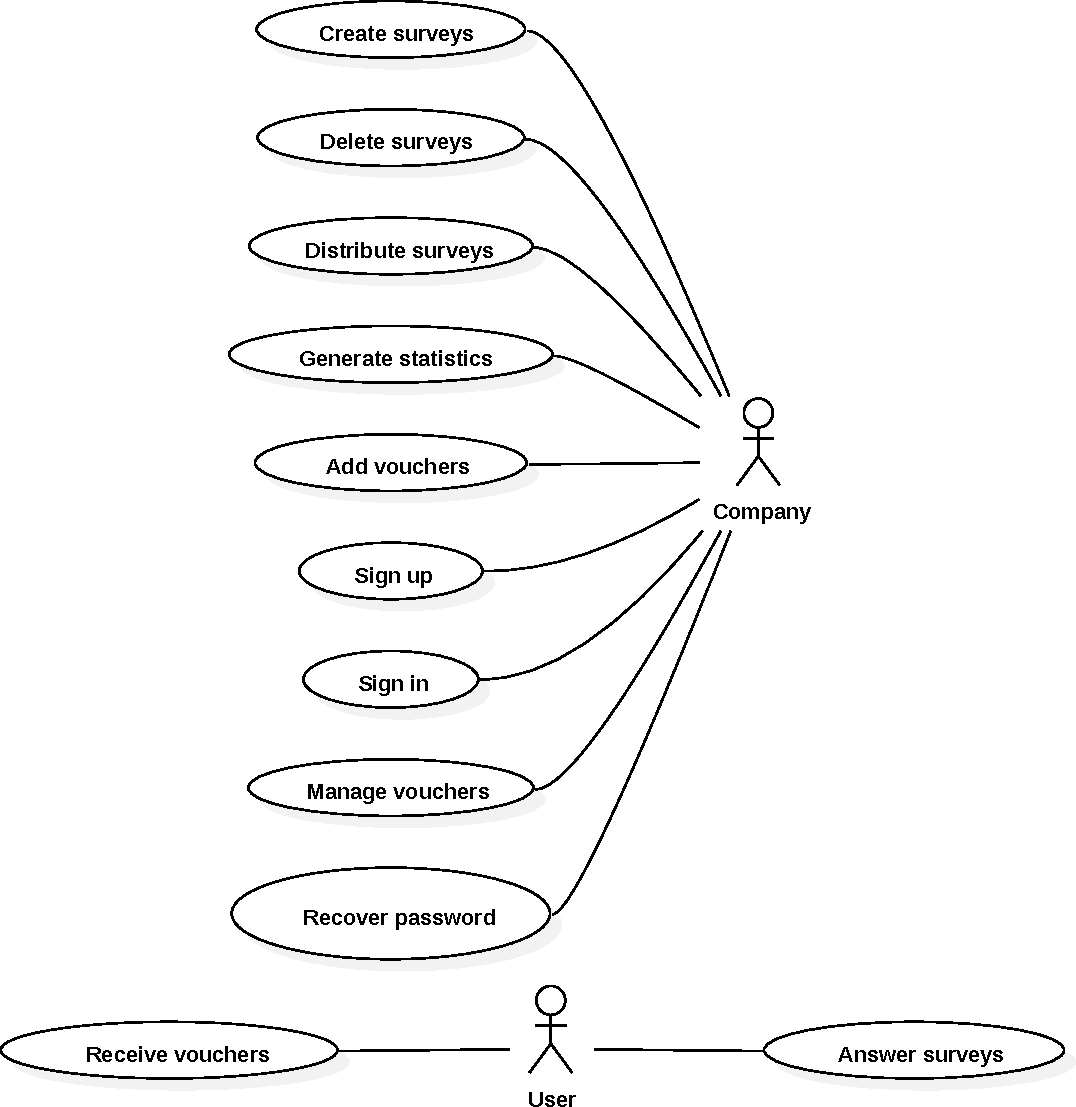
\includegraphics[width=10cm,height=10cm,keepaspectratio]{useCasePdf}
\caption{Diagram przypadków użycia dla systemu.}
\end{figure}

\paragraph{}
W dalszej części dokumentacji będą używane terminy, których znaczenie znajduje swój odpowiednik w modelu systemu. Terminy te zostaną teraz opisane dla zwiększenia czytelności i jasności dokumentacji:
\begin{itemize}
\item \textbf{Ankieta} - zbiór pytań otwartych, ze skalą lub jednokrotnego/wielokrotnego wyboru.
\item \textbf{Kupon} - zniżka na konkretny produkt lub usługę.
\item \textbf{Kod promocyjny} - kod powiązany z kuponem, uprawniający do zniżki na konkretny produkt lub usługę.
\end{itemize}
\clearpage

\chapter{Analiza problemu}

\paragraph{}
Podobną funkcjonalność do opisywanego w dokumentacji systemu ma aplikacja webowa \textit{surveybee.net}. Oferuje ona nagrody pieniężne za wypełnienie ankiety, jednak minimalna stawka zarobionych pieniędzy, pozwalająca na wypłatę sprawia, że wypełniający musiałby poświęcić dużo czasu, aby otrzymać swoją nagrodę. Nasz system pozwala na natychmiastowe otrzymanie nagrody w postaci kuponu, bezpośrednio po wypełnieniu ankiety.

\paragraph{}
Innym systemem, znacznie bardziej popularnym i posiadającym większą reputację jest \textit{surveymonkey.com}. System ten pozwala firmom na tworzenie ankiet, które następnie mogą być wypełniane przez użytkowników. Aplikacja ta nie pozwala jednak na wprowadzenie gratyfikacji w zamian za wypełnienie ankiety.

\paragraph{}
Nasz system posiada zatem założenia funkcjonalne, którym różni się od produktów dostępnych na rynku. Implementacja takich założeń wiązała się z rozwiązaniem kilku problemów, które umożliwiałyby efektywne i bezpieczne wprowadzenie wspomnianych w rodziale pierwszym funkcjonalności.


\subsection{Problem liczby kuponów}
\paragraph{}
Jednym z najważniejszych założeń funkcjonalnych naszego systemu jest przekazywanie użytkownikom kuponów w zamian za wypełnienie ankiety. Problem ten jest trudny w sytuacji, gdy ilość kodów promocyjnych powiązanych z kuponami jest ograniczona. W przypadku naiwnego rozwiązania, polegającego na przydzielaniu kuponu wypełniającemu w momencie kliknięcia przycisku \texttt{Wyślij}, mogłoby dojść do sytuacji, w której ostatni kod zostałby przydzielony osobie, która szybciej rozwiązała ankietę. Osoba, która rozwiązywałaby ankietę wolniej po kliknięciu przycisku \texttt{Wyślij} zostałaby poinformowana o braku kodu promocyjnego. Jej czas przeznaczony na wypełnienie ankiety nie zostałby więc nagrodzony, a sam wypełniający poczułby się oszukany.

\paragraph{}
Aby uniknąć takiej sytuacji wprowadzone zostało blokowanie kuponów, które jest połączone z sesją użytkownika. Użytkownik po wybraniu interesującej go ankiety ma wiązany swój identyfikator sesji z kodem promocyjnym. W przypadku braku kodów promocyjnych dla danego kuponu, ankieta nie będzie widoczna dla użytkowników w systemie do momentu dodania większej ilości kodów promocyjnych. Dzięki takiemu rozwiązaniu użytkownik ma gwarancję otrzymania nagrody już na początku wybrania ankiety. Takie rozwiązanie wiąże się również z możliwościami paraliżowania systemu przez złośliwych użytkowników. W negatywnym przypadku złośliwy użytkownik mógłby zablokować wszystkie kody promocyjne dla siebie, przez co ankieta stałaby się niewidoczna dla innych użytkowników. Aby zapobiec takiej sytuacji wprowadzone zostały stosowne zabezpieczenia. Użytkownik systemu może w danym momencie mieć tylko jeden kod promocyjny powiązany z identyfikatorem sesji. Powiązanie te jest aktywne w systemie tylko przez 15 minut. Ponadto zamknięcie ankiety poprzez naciśnięcie przycisku \texttt{Anuluj} spowoduje zwrócenie kodu promocyjnego do puli. Dokładny opis procesu blokowania kuponu jest opisany w rodziale czwartym.

\subsection{Problem anonimowości}
\paragraph{}
W trosce o rzetelność odpowiedzi system zapewnia anonimowość odpowiadających. W bazie danych nie są przechowywane żadne dane osobowe, pozwalające na jednoznaczne zidentyfikowanie wypełniającego ankietę. Wszystkie dane osobowe, które mogą jednoznacznie wiązać użytkownika z konkretną osobą nie są przechowywane w bazie i są całkowicie opcjonalne. Przykładem takich danych jest adres e-mail, na który może zostać wysłany kupon po wypełnieniu ankiety. Jest on podawany opcjonalnie po wypełnieniu ankiety i nie jest nigdzie przechowywany. Innymi danymi zbieranymi od użytkownika są wiek oraz kraj pochodzenia, jednak informacje takie nie pozwalają wnioskować jednoznacznie o tożsamości wypełniającego.

\subsection{Problem bezpieczeństwa}
\paragraph{}
W systemie, który jako główne założenie funkcjonalne oferuje wartość materialną w zamian za wypełnienie ankiety, ważne jest zapewnienie bezpieczeństwa. Pierwszym problemem była walidacja odpowiedzi na ankiety. System należało zabezpieczyć przed atakami XSS zarówno przeprowadzanymi ze strony wypełniającego, jak i firmy. Aby ich uniknąć, wszystkie przesyłane pytania i odpowiedzi są walidowane przez serwer. Jako dodatkową walidację, zostało wprowadzone sprawdzanie tworzonych ankiet od strony front-endu. Nie jest to jednak zabezpieczenie wystarczające, aby uniemożliwić takie ataki, gdyż rozwiązania front-endowe mogą być modyfikowane od strony klienta. System jest również zabezpieczony przed atakami typu CSRF poprzez użycie tokenów CSRF. Szczegóły tego rozwiązania zostały opisane w rodziale trzecim. Zabezpieczone zostały również komponenty systemu, do których dostęp powinny mieć tylko zalogowane firmy, dzięki zastosowaniu podziału na role i autoryzacji w systemie. To rozwiązanie również zostało opisane dokładnie w rodziale trzecim. Dane firmy przechowywane są w bazie danych w sposób minimalizujący straty w razie ewentualnego wycieku danych. Hasła firm trzymane są w postaci hasha z solą, dzięki czemu adwersarz porównujący hasła nie jest w stanie stwierdzić identyczności między hasłami poszczególnych firm. Również proces odzyskiwania hasła został zaprojektowany w sposób bezpieczny, który uniemożliwia przejęcie kontroli nad kontem firmowym osobie trzeciej.

\chapter{Projekt}
\subsection{Architektura projektu}
Cieżko jest mówić o naszej aplikacji jak o jednym bycie, ponieważ można ją podzielić na dwa podsystemu, gdzie w obu przypadkach archiktektura systemu jest wielowarstwowa. Jednym z podsystemów jest aplikacja webowa, która została zaprojektowana w oparciu o wzorzec \textbf{MVC} (ang. Model-View-Controller), który to narzucił wielowarstwową architektura. Oddzielając logikę biznesową od modelu (tj. danych) oraz interfejsu użytkownika aplikacji została zaprojektowana zgodnie z zasadami \textbf{GRASP} (ang. General responsibility assignment software patterns). Taka a nie inna architektura aplikacji webowej oprócz znacznego zwiększenia czytelności kodu pozwoliła na wielowarstwowe zabezpieczenia, które zostały nałożone na każdą z trzech głównych warstw naszej aplikacji. Samą część łącząca wartswe modelu oraz controller'a możemy podzielić na dwie podwarstwy: \textbf{DAO} (ang. Data Access Object) oraz \textbf{Service}.
\begin{figure}[H]
  \centering
  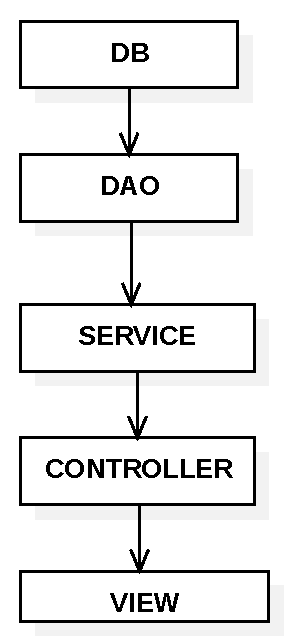
\includegraphics[scale=0.6]{diagram1.pdf}
  \caption{System podzielony na podwarstwy.}
\end{figure}
Warstwa \textbf{DAO} odpowiedzialna jest bezpośrednio na komunikacje z wartswą modelu, tj. bazą danych. Natomiast to w warstwie serwisowej, która korzysta z warstwy \textbf{DAO} została zaimplementowana cała logika biznesowa i to właśnie z warstwy serwisowej korzystamy w kontrolerach.

\paragraph{}
Drugim podsystemem naszego projektu jest aplikacja webowa, która również jest systemem rozproszonym komunikującym się z serwerem (który jest częścią pierwszego podsystemu) wykorzystując \textbf{REST} (ang. Representational State Transfer) oferując użytkownikowi jedynie część funkcjonalności aplikacji webowej.

\paragraph{}
W projekcie poza stosowaniem zasad \textbf{GRASP} zostały wykorzystane takie wzorce projektowe jak \textbf{Proxy}, \textbf{Template Method}, \textbf{Adapter}, \textbf{Factory} oraz \textbf{Decorator}, \textbf{Dependency Injection}, \textbf{Aspect Oriented Programing}, \textbf{Singleton}, które w sposób naturalny współgrały z użytymi przez nas technologiami.
\subsection{Przypadki użycia i scenariusze}
\begin{table}[H]
	\centering
	\sffamily\captionsetup{justification=raggedright,singlelinecheck=false,position = below, font = sf}
	\begin{tabular}{|m{3.5cm}|m{11cm}|}
	\hline 
	UC1 & Add Survey \\
	\hline
	Actors & Company \\ 
	\hline
	Preconditions & Company is signed in and is in the dashboard page. \\
	\hline
	Postconditions & Company added survey. \\
	\multirow{6}{*}{Main Success Scenario} & 1.Company hits on 'Add Survey' button. \\
	\cline{2-2}
	& 2.Company hits proper 'Add Question' button depending on what type of question company wants. \\
	\cline{2-2}
	& 3.Company fills up question's content. \\
	\cline{2-2}
	& 4.Company repeats steps from point 2. until completes survey. \\
	\cline{2-2}
	& 5.Company hits 'Add Voucher' button in order to compose survey with concere voucher. \\
	\cline{2-2}
	& 6.Company hits 'Confirm Survey' button. \\
	\hline
	\multirow{4}{*}{Alternate flows} & 2a.Company hits 'Confirm Survey' button without adding any questions: \\
	\cline{2-2}
	& \multicolumn{1}{c|}{1.System signals error and doesn't proceed.} \\
	\cline{2-2}
	& 5a.Company hits 'Confirm Survey' button without adding voucher: \\
	\cline{2-2}
	& \multicolumn{1}{c|}{1.System signals error and doesn't proceed.} \\
	\hline	
	\end{tabular}
\end{table}		

\paragraph{}
Powyższy przypadek użycia opisuje proces dodawania ankiety so systemu. Szczegóły dodawania ankiety zostały opisane w rozdziale czwartym.
		
\begin{table}[H]
	\centering
	\sffamily\captionsetup{justification=raggedright,singlelinecheck=false,position = below, font = sf}
	\begin{tabular}{|m{3.5cm}|m{11cm}|}
	\hline
	UC2 & Sign in \\
	\hline
	Actors & Company \\
	\hline
	Preconditions & Company is registered in the System  \\
	\hline
	Postconditions & Company is signed in. \\
	\hline
	\multirow{7}{*}{Main Success Scenario} & 1.Company enters the website and is on landing page \\
    \cline{2-2}
     & 2.Company hits the Sign In button. \\
	\cline{2-2}
     & 3.System moves the Company to the Sign In page.\\
	\cline{2-2}
     & 4.Company enters the login. \\
	\cline{2-2}
     & 5.Company enters the password. \\
	\cline{2-2}
     & 6.Company hits the Sign In/Enter button. \\
	\cline{2-2}
     & 7.System moven the Company to the dashboard page. \\
    \hline
    \multirow{10}{*}{Alternate flows} & 2a.Company hits the Sign Up button: \\
	\cline{2-2}
	& \multicolumn{1}{c|}{1.System moves the Company to the Sign Up page.} \\
	\cline{2-2}
	& 6a.Company hits the Sign Up button or "Doesn't hvae an account? Create one here now!" text. \\
	\cline{2-2}
	& \multicolumn{1}{c|}{1.System moves the Company to the Sign Up page.}	 \\
	\cline{2-2}
	& 6b.Company hits "Forgot the password" text. \\
	\cline{2-2}
	& \multicolumn{1}{c|}{1.Company is guided through password recovery process.} \\
	\cline{2-2}
	& 7a.Invalid login: \\
	\cline{2-2}
	& \multicolumn{1}{c|}{1.System signals error and doesn't proceed/stays on the Sign In page.}	 \\
	\cline{2-2}
	& 7b.Invalid password: \\
	\cline{2-2}
	& \multicolumn{1}{c|}{1.System signals error and doesn't proceed/stays on the Sign In page.} \\
    \hline
	\end{tabular}
\end{table}

\paragraph{}
Powyższy przypadek użycia opisuje proces logowania do systemu. Szczegółowy proces został opisany w rozdziale czwartym.
	
	\begin{table}[H]
	\centering
	\sffamily\captionsetup{justification=raggedright,singlelinecheck=false,position = below, font = sf}
	\begin{tabular}{|m{3.5cm}|m{11cm}|}
	\hline 
	UC3 & Sign up \\
	\hline
	Actors & Company \\
	\hline
	Preconditions & Company is not already registered in the System. \\
	\hline
	Postconditions & Company is registered in the System. Company is able to access its dashboard. \\	
	\hline
	\multirow{8}{*}{Main Success Scenario} & 1.Company enters the website and is on landing page. \\
	\cline{2-2}
	& 2.Company hits the Sign Up button. \\
	\cline{2-2}
	& 3.System moves the Company to the Sign Up page. \\
	\cline{2-2}
	& 4.Company enters login, password, name and address. \\
	\cline{2-2}
	& 5.Company hits Sign Up/Enter button. \\
	\cline{2-2}
	& 6.System notifies Company about successful registration. \\
	\cline{2-2}
	& 7.System moves Company to the landing page. \\
	\cline{2-2}
	& 8. System can also demand entering a verification token from e-mail after the registration. \\
	\hline
	\multirow{10}{*}{Alternate flows} & 2a.Company hits the Sign In button: \\
	\cline{2-2}
	& \multicolumn{1}{c|}{1.System moves the Company to the Sign In page.} \\
	\cline{2-2}
	& 5a.Company hits Cancel/Back button: \\
	\cline{2-2}
	& \multicolumn{1}{c|}{1.System moves the Company to the landing page.} \\
	\cline{2-2}
	& 6a.Login/e-mail already taken: \\
	\cline{2-2}
	& \multicolumn{1}{c|}{1.System signals error and doesn't proceed.} \\
	\cline{2-2}
	& 6b.Login/Name/Address contains forbidden symbols: \\
	\cline{2-2}
	& \multicolumn{1}{c|}{1.System signals error, suggests the proper symbol range and doesn't proceed.} \\
	\cline{2-2}
	& 6c.Any of registration fields is empty: \\
	\cline{2-2}
	& \multicolumn{1}{c|}{1.System signals error, suggests to fill the empty field and doesn't proceed.} \\
	\hline
	\end{tabular}
	\end{table}
	
\paragraph{}
Powyższy przypadek użycia opisuje proces rejestracji w systemie. Szczegółowy proces został opisany w rozdziale czwartym.
	
	\begin{table}[H]
	\centering
	\sffamily\captionsetup{justification=raggedright,singlelinecheck=false,position = below, font = sf}
	\begin{tabular}{|m{3.5cm}|m{11cm}|}
	\hline 
	UC4 & Filling up the survey \\
	\hline
	Actors & User \\ 
	\hline
	Preconditions & None or the mobile app installed required , if user want's to make it that way \\
	\hline
	Postconditions & User accomplished fulfilling the survey. User gain a voucher code. \\
	\multirow{10}{*}{Main Success Scenario} & 1.User chose a company, which voucher might be interesting for him (either in mobile app or website). \\
	\cline{2-2}
	& 2.System moves user to website where the survey is shown. \\
	\cline{2-2}
	& 3.User fulfilss whole survey step by step. \\
	\cline{2-2}
	& 4.User hits 'Done' button. \\
	\cline{2-2}
	& 5.System validates survey and user moves forward. \\
	\cline{2-2}
	& 6.System notifies user that the survey is accepted. \\
	\cline{2-2}
	& 7.System asks user for e-mail Adress	 \\
	\cline{2-2}
	& 8.User can aceppt his e-mail Adress by pressing the button.  \\
	\cline{2-2}
	& 9.System sends voucher to user. \\
	\cline{2-2}
	& 10.System notifies user that the voucher has been sent. \\
	\hline
	\multirow{3}{*}{Alternate flows} & 5a.Survey rejected, validation didn't pass: \\
	\cline{2-2}
	& \multicolumn{1}{c|}{1.Special informations are displayed.} \\
	\cline{2-2}
	& \multicolumn{1}{c|}{2.User is asked to fix his answers.} \\
	\cline{2-2}
	\multirow{3}{*}{Alternate flows} & 9a.User passed e-mail that don't match e-mail address' pattern: \\
	\cline{2-2}
	& \multicolumn{1}{c|}{1.Special informations are displayed.} \\
	\cline{2-2}
	& \multicolumn{1}{c|}{2.User is asked to pass proper e-mail address.} \\
	\hline	
	\end{tabular}
	\end{table}	

\paragraph{}
Powyższy przypadek użycia opisuje proces wypełniania ankiety. Szczegółowy proces został opisany w rozdziale czwartym.
	
	
	\begin{table}[H]
	\centering
	\sffamily\captionsetup{justification=raggedright,singlelinecheck=false,position = below, font = sf}
	\begin{tabular}{|m{3.5cm}|m{11cm}|}
	\hline 
	UC5 & Add Voucher \\
	\hline
	Actors & Company \\
	\hline
	Preconditions & Company is signed in and is in dashboard page. \\
	\hline
	Postconditions & Company added voucher. \\	
	\hline
	\multirow{5}{*}{Main Success Scenario} & 1.Company hits „Add voucher” button. \\
	\cline{2-2}
	& 2.Company fills up voucher details( some details in plain text,type of discount, discount rate etc.) \\
	\cline{2-2}
	& 3.Company hits „Add voucher” button to add voucher to right survey from dropdown list. \\
	\cline{2-2}
	& 4.Company confirms voucher by „Confirm voucher” button. \\
	\cline{2-2}
	& 5.Voucher is added. \\
	\hline
	\multirow{6}{*}{Alternate flows} & 5a. Voucher already exist: \\
	\cline{2-2}
	& \multicolumn{1}{c|}{1.Proper error message is displayed.} \\
	\cline{2-2}
	& \multicolumn{1}{c|}{2.Filled for is displayed, company is asked to pass diffrent voucher.} \\
	\cline{2-2}
	& 5b.Company didn't pick any survey: \\
	\cline{2-2}
	& \multicolumn{1}{c|}{1.Proper error message is displayed.} \\
	\cline{2-2}
	& \multicolumn{1}{c|}{2.Filled for is displayed, company is asked to pass diffrent voucher.} \\
	\cline{2-2}
	\hline
	\end{tabular}
	\end{table}
	
\paragraph{}
Powyższy przypadek użycia opisuje proces dodawania kuponu. Szczegółowy proces został opisany w rozdziale czwartym.
	
	\begin{table}[H]
	\centering
	\sffamily\captionsetup{justification=raggedright,singlelinecheck=false,position = below, font = sf}
	\begin{tabular}{|m{3.5cm}|m{11cm}|}
	\hline 
	UC6 & Remove account \\
	\hline
	Actors & Company \\
	\hline
	Preconditions & Company is registered in system. \\
	\hline
	Postconditions & Company doesn’t have an account. \\	
	\hline
	\multirow{5}{*}{Main Success Scenario} & 1.Company hits „Delete account” button \\
	\cline{2-2}
	& 2.Confirmation window appears asking for confirmation. \\
	\cline{2-2}
	& 3.Company confirms the action by entering the password to the site. \\
	\cline{2-2}
	& 4.All information about the company, surveys and coupons are deleted from database. \\
	\cline{2-2}
	& 5.Company sees statement „Your account has been deleted.”. \\
	\hline
	\end{tabular}
\end{table}

\paragraph{}
Powyższy przypadek użyca opisuje proces usuwania konta z systemu. Wraz z usunięciem konta z systemu, z bazy danych są usuwane kaskadowo wszystkie krotki, które były powiązane z danym kontem firmowym.


\subsection{Diagramy klas}
Diagramy przedstawione poniżej przedstawiają klasy serwisowe, w których to właśnie została zaimplementowana cała logika biznesowa naszego systemu  i to one reprezentują funkcjonalność i możliwości naszej aplikacji webowej. W celu zwiększenia czytelności diagramów z ich większości zostały usunięte trywialne metody (nie zawierające logiki biznesowej), których zadaniem było dodanie, edycja, usunięcie przekazywanego obiektu w bazie danych.
\begin{figure}[H]
  \centering
  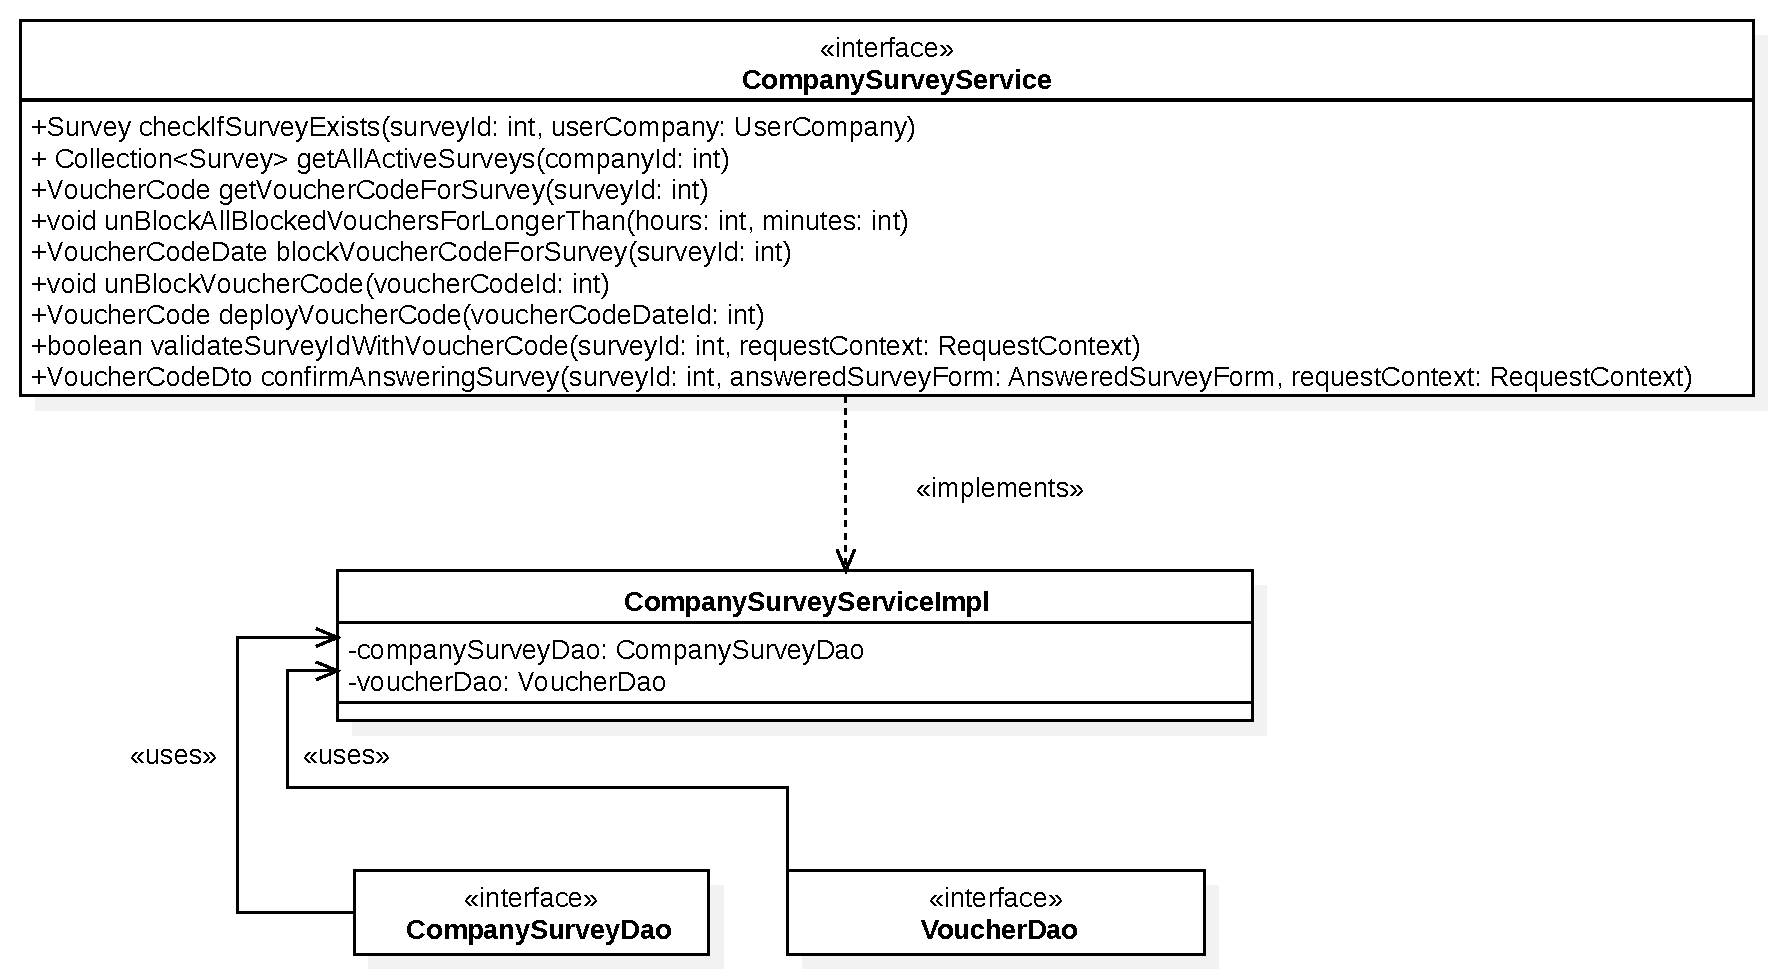
\includegraphics[width=15cm,height=20cm,keepaspectratio]{company_survey_service.pdf}
  \caption{Diagram klas dla interfejsu serwisowego $CompanySurveyService$}
\end{figure}
Powyższy diagram przedstawia diagram klas dla serwisu, który przede wszystskim obsługuje funkcjonalność związana pobieraniem aktywnym, przeglądaniem oraz wypełnianiem ankiet jak również walidacją tych czynności. Ponadto odpowiedzialny jest za podjęcie decyzji czy dany kupon powininen zostać wydany czy też nie.
\begin{figure}[H]
  \centering
  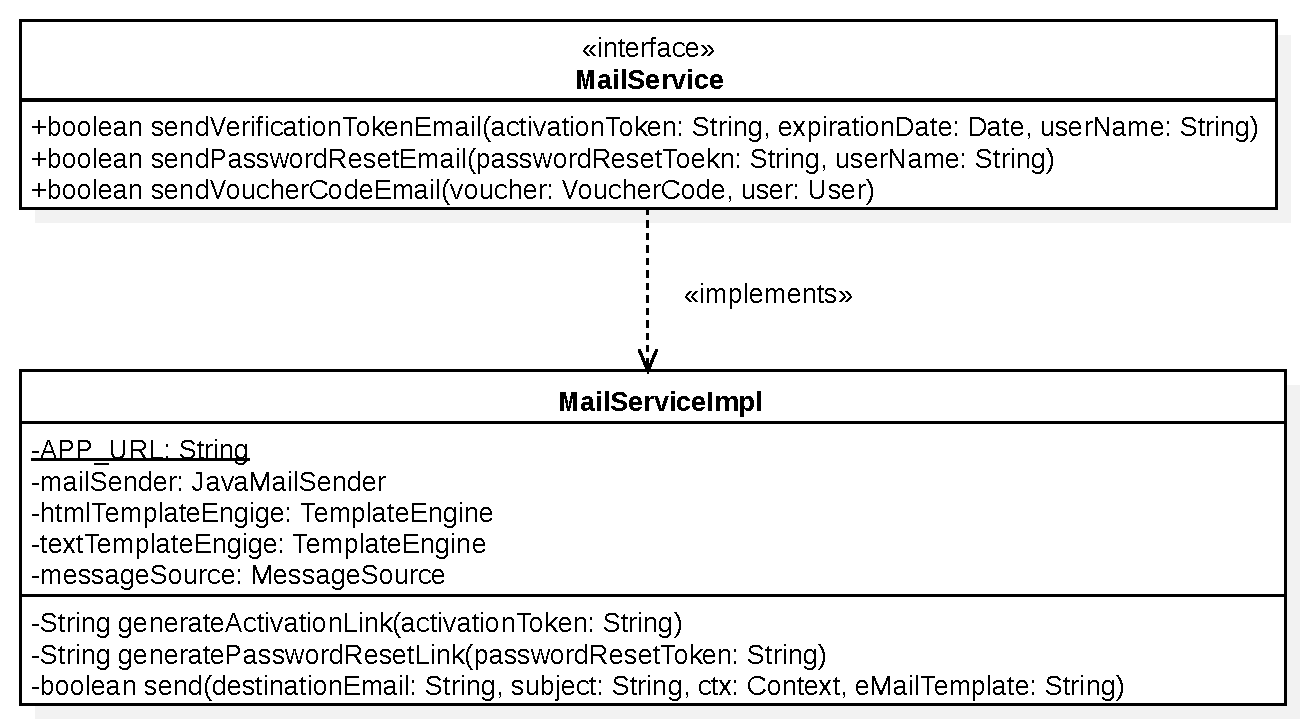
\includegraphics[scale=0.6]{mail_service.pdf}
  \caption{Diagram klas dla interfejsu serwisowego $MailService$}
\end{figure}
W \textbf{MailService} każda metoda odpowiada innemu typu  wiadomości, która zostanie wysłąna.
\begin{figure}[H]
  \centering
  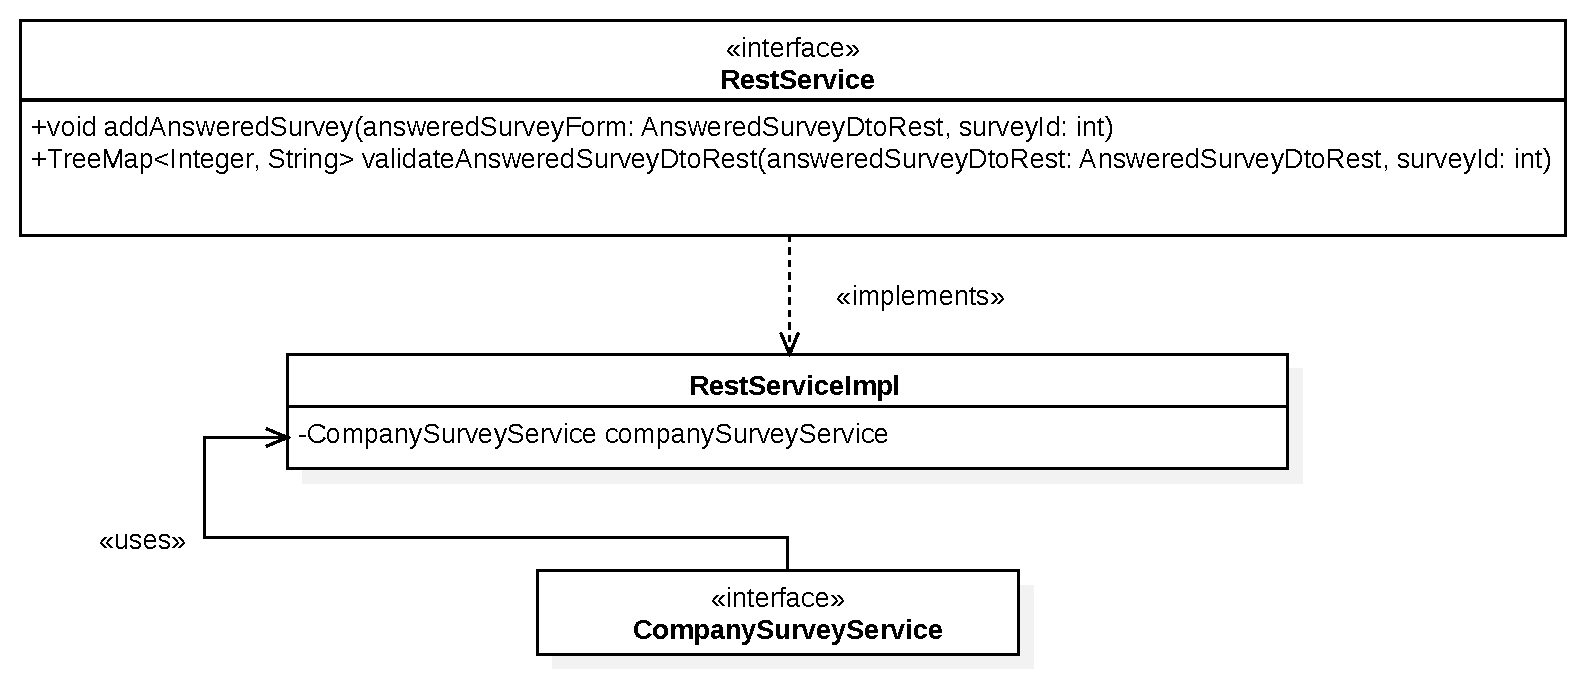
\includegraphics[scale=0.6]{rest_service.pdf}
  \caption{Diagram klas dla interfejsu serwisowego $RestService$}
\end{figure}
Powyższy diagram klas przedstawia diagram klas serwisowych obsługujących \textbf{REST Api}, które jest wykorzystywane przez aplikacje mobilna.
\begin{figure}[H]
  \centering
  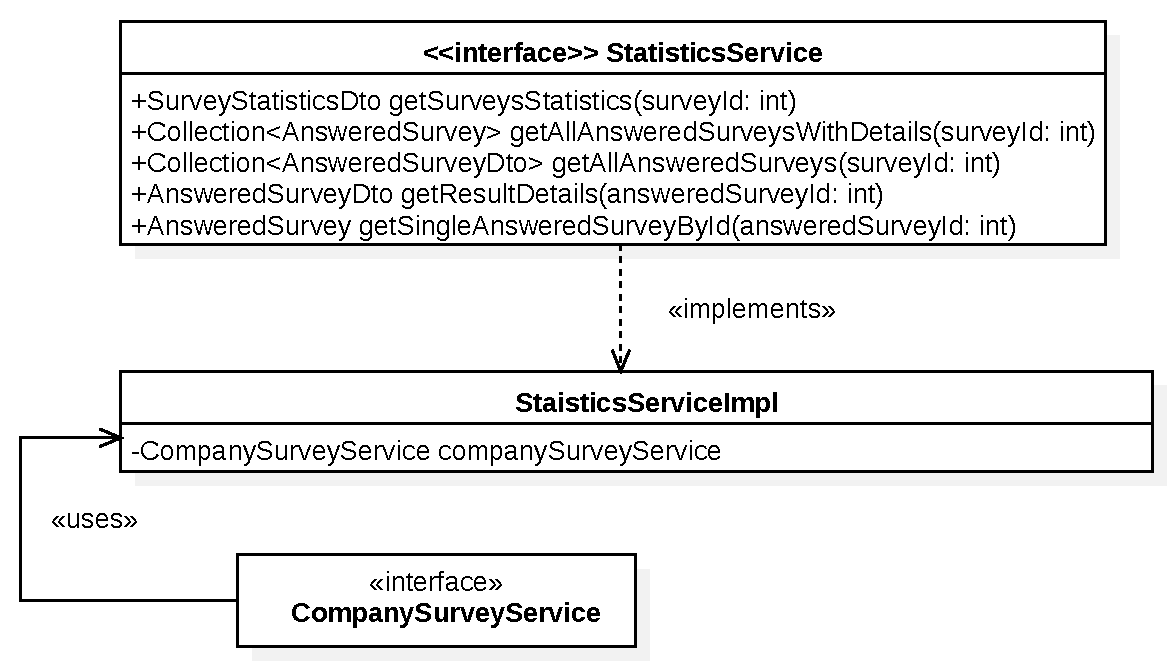
\includegraphics[scale=0.6]{statistics_service.pdf}
  \caption{Diagram klas dla interfejsu serwisowego $StatisticsService$}
\end{figure}
W powyżej przedstawionych klasach serwisowych obliczane są statystyki, które każdy użytkownik ze stworzonymi ankietami może przeglądać.
\begin{figure}[H]
  \centering
  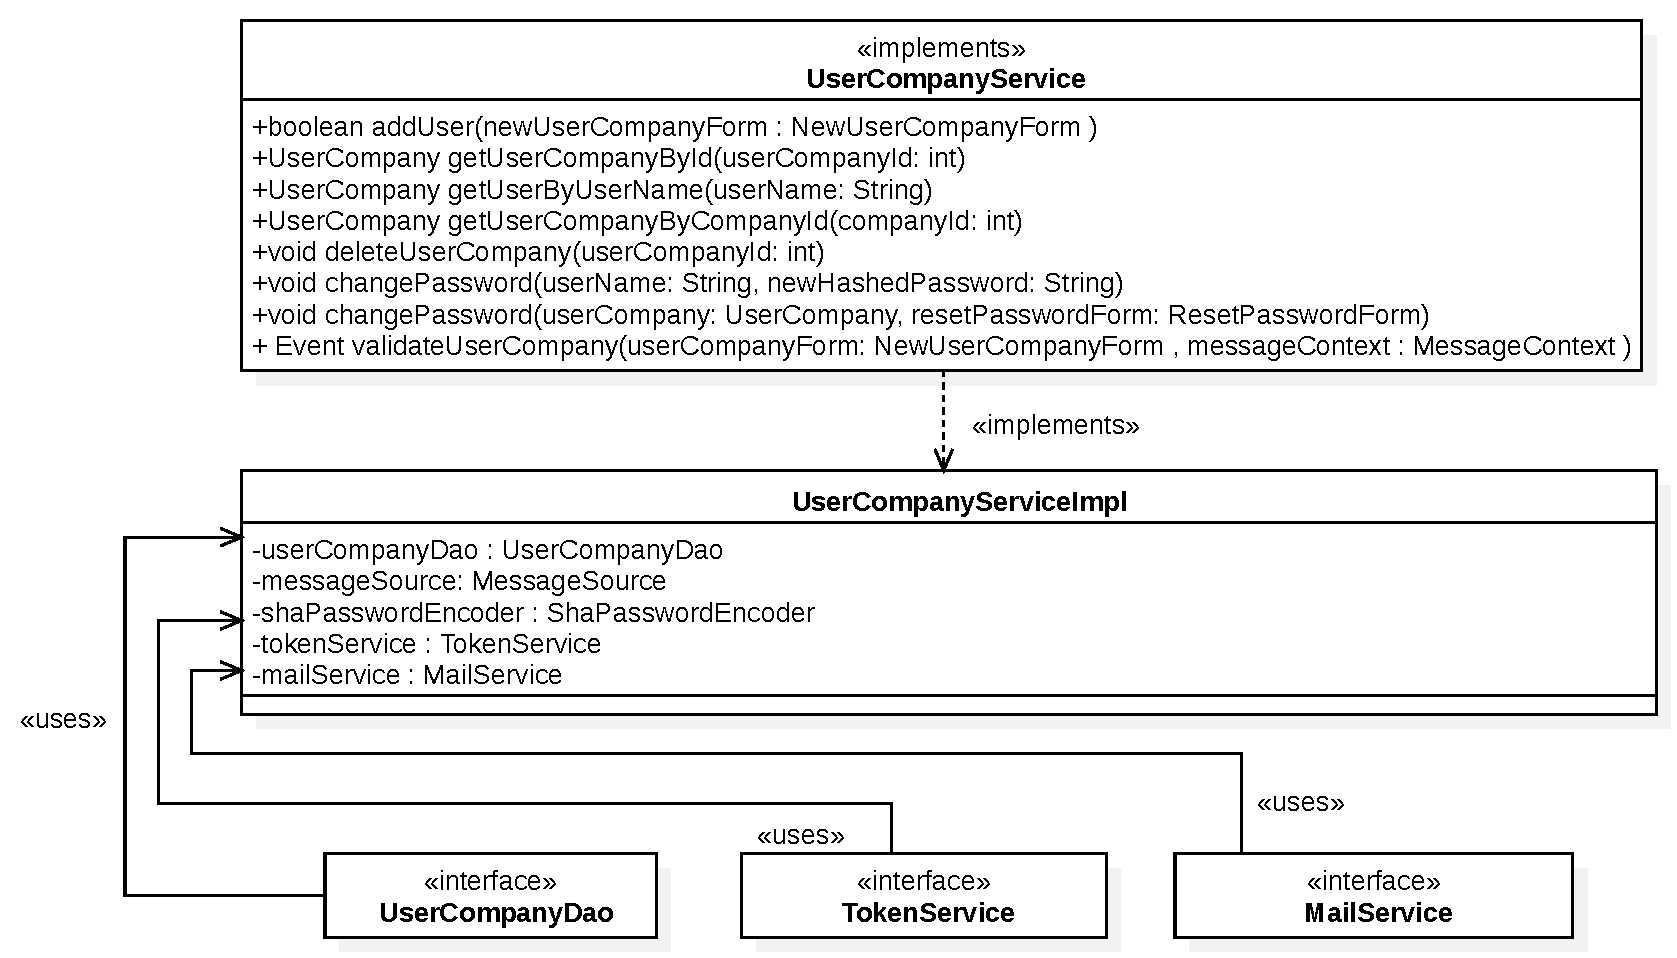
\includegraphics[width=12cm,height=17cm,keepaspectratio]{user_company_service.pdf}
  \caption{Diagram klas dla interfejsu serwisowego $UserCompanyService$.}
\end{figure}
Klasy serwisowe w diagramie powyżej odpowiadają za część funckjonalności związanej z kontem firmy, tj. edycja danych, rejestracja, logowanie, zmiana hasła itd.
\subsection{Diagramy aktywności}
\begin{figure}[htbp]
  \centering
  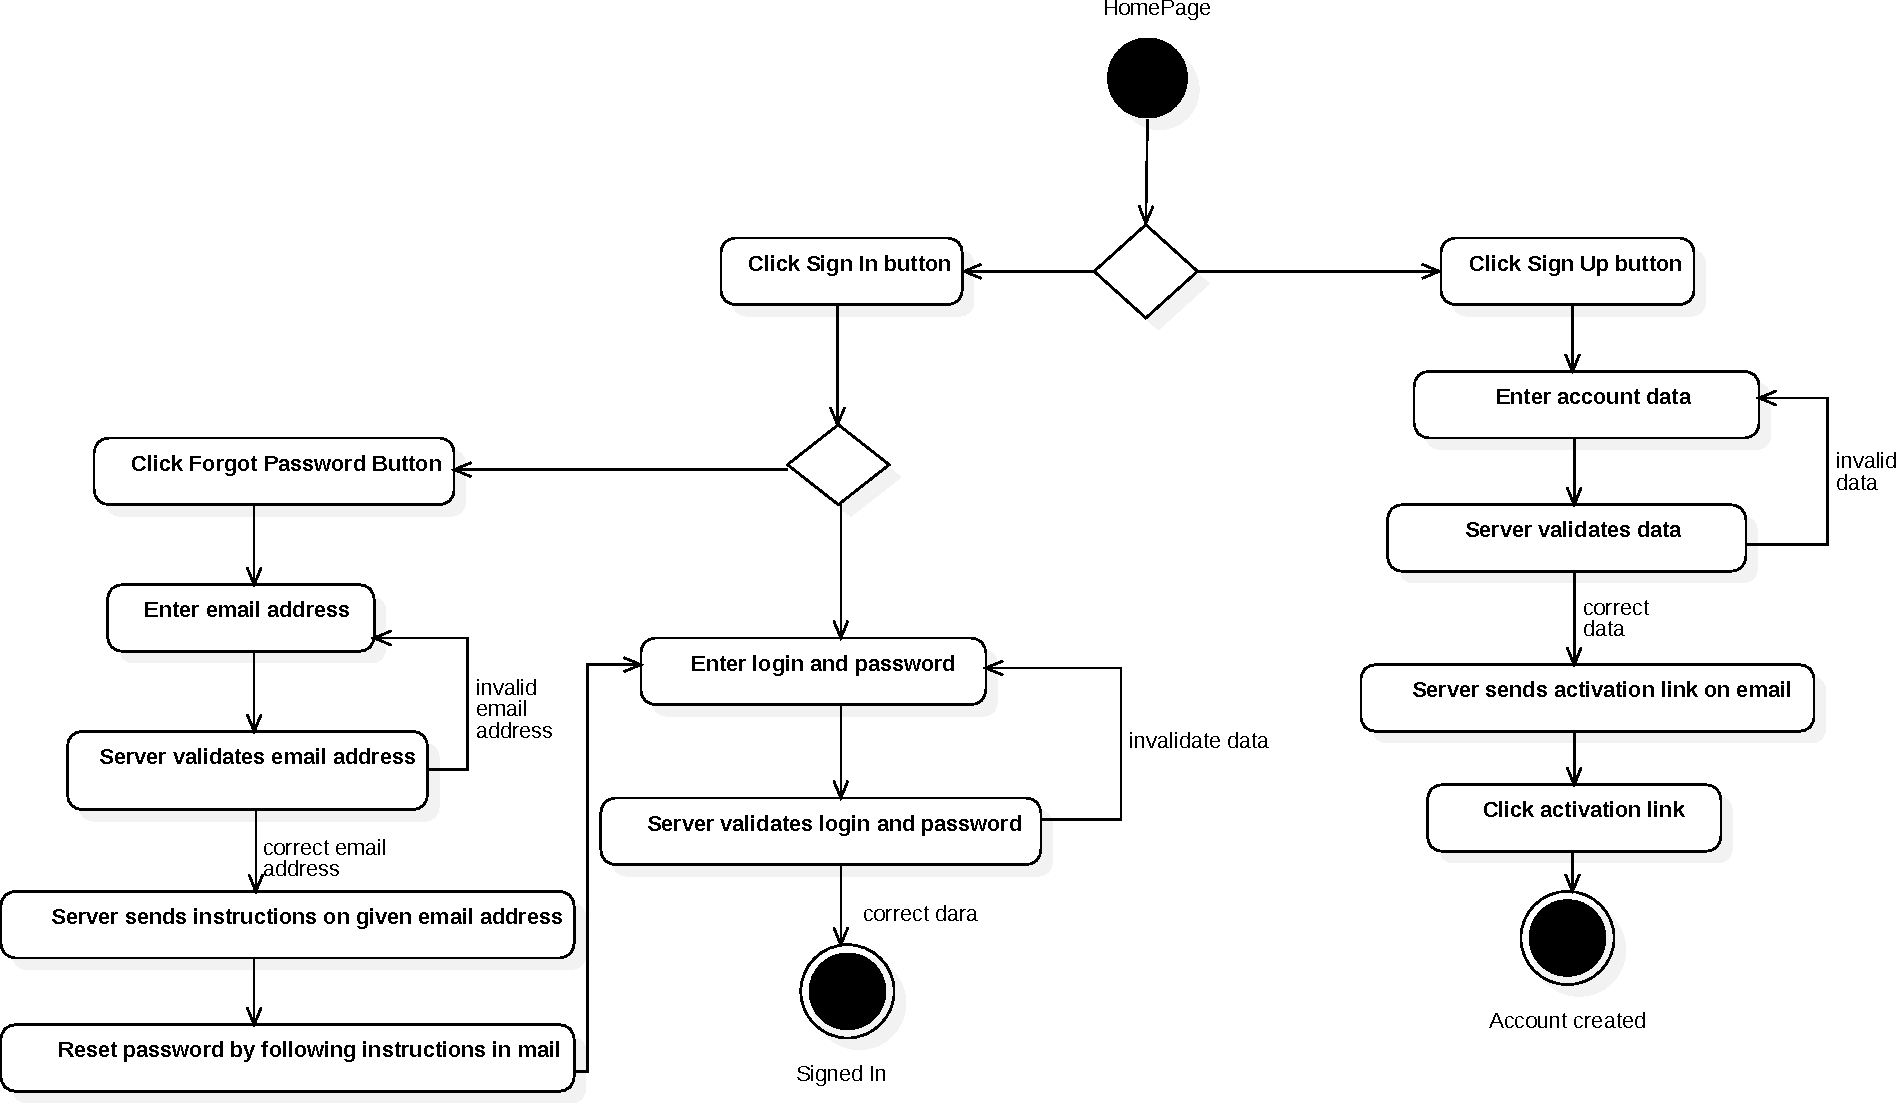
\includegraphics[scale=0.5]{activitySISU.pdf}
  \caption{Diagram aktywności dla logowania i rejestracji.}
\end{figure}

\paragraph{}
Powyższy diagram aktywności opisuje proces logowania i rejestracji w aplikacji webowej. Szczegółowy opis został przedstawiony w rodziale czwartym.

\begin{figure}[htbp]
  \centering
  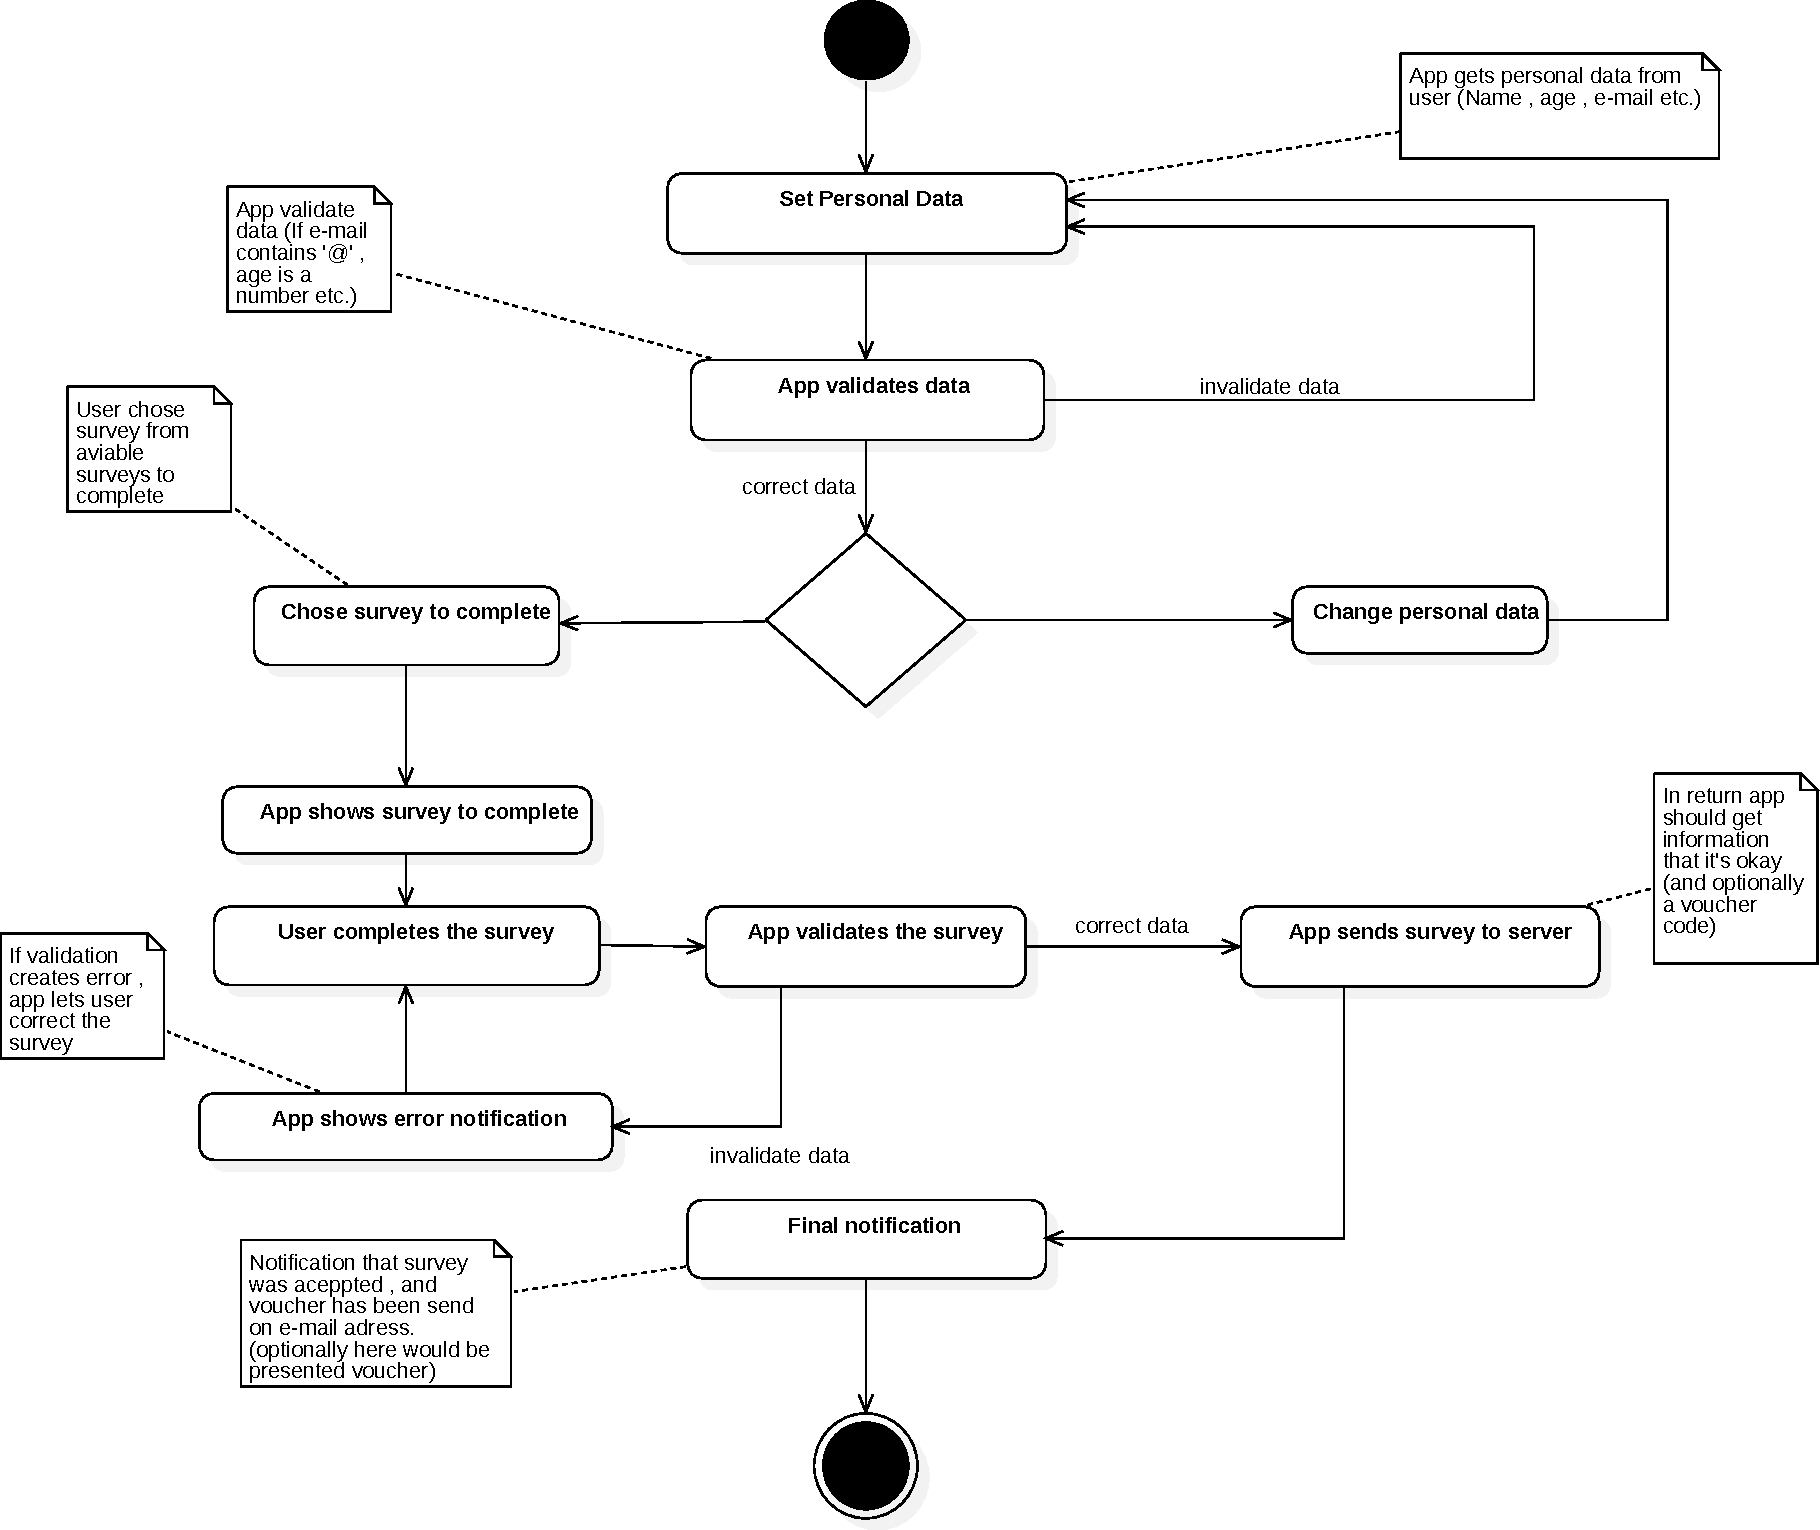
\includegraphics[scale=0.4]{MobileAppActivityDiagram.pdf}
  \caption{Diagram aktywności dla aplikacji mobilnej.}
\end{figure}

\paragraph{}
Głównym celem aplikacji mobilnej dla naszego serwisu, było umożliwienie użytkownikom w łatwy i prosty sposób uzupełnianie ankiet, oraz otrzymywanie kuponów w taki sposób, aby np. móc je okazać w sklepie na urządzeniu mobilnym. Przy pierwszym uruchomieniu aplikacji, użytkownik jest proszony o wprowadzenie danych dla celów statystyki. Jest to komfortowe rozwiązanie dla tych użytkowników, którzy planują korzystać z naszej aplikacji więcej niż raz. Aplikacja następnie wyświetla listę dostępnych firm oraz ankiet. Dzięki korzystaniu z aplikacji, użytkownik ma pod ręką możliwość wypełnienia dowolnej z możliwych ankiet w każdym momencie oraz dostęp do swoich wszystkich otrzymanych i niewykorzystanych kuponów.

\pagebreak
\subsection{Projekt bazy danych}
\begin{figure}[H]
  \centering
  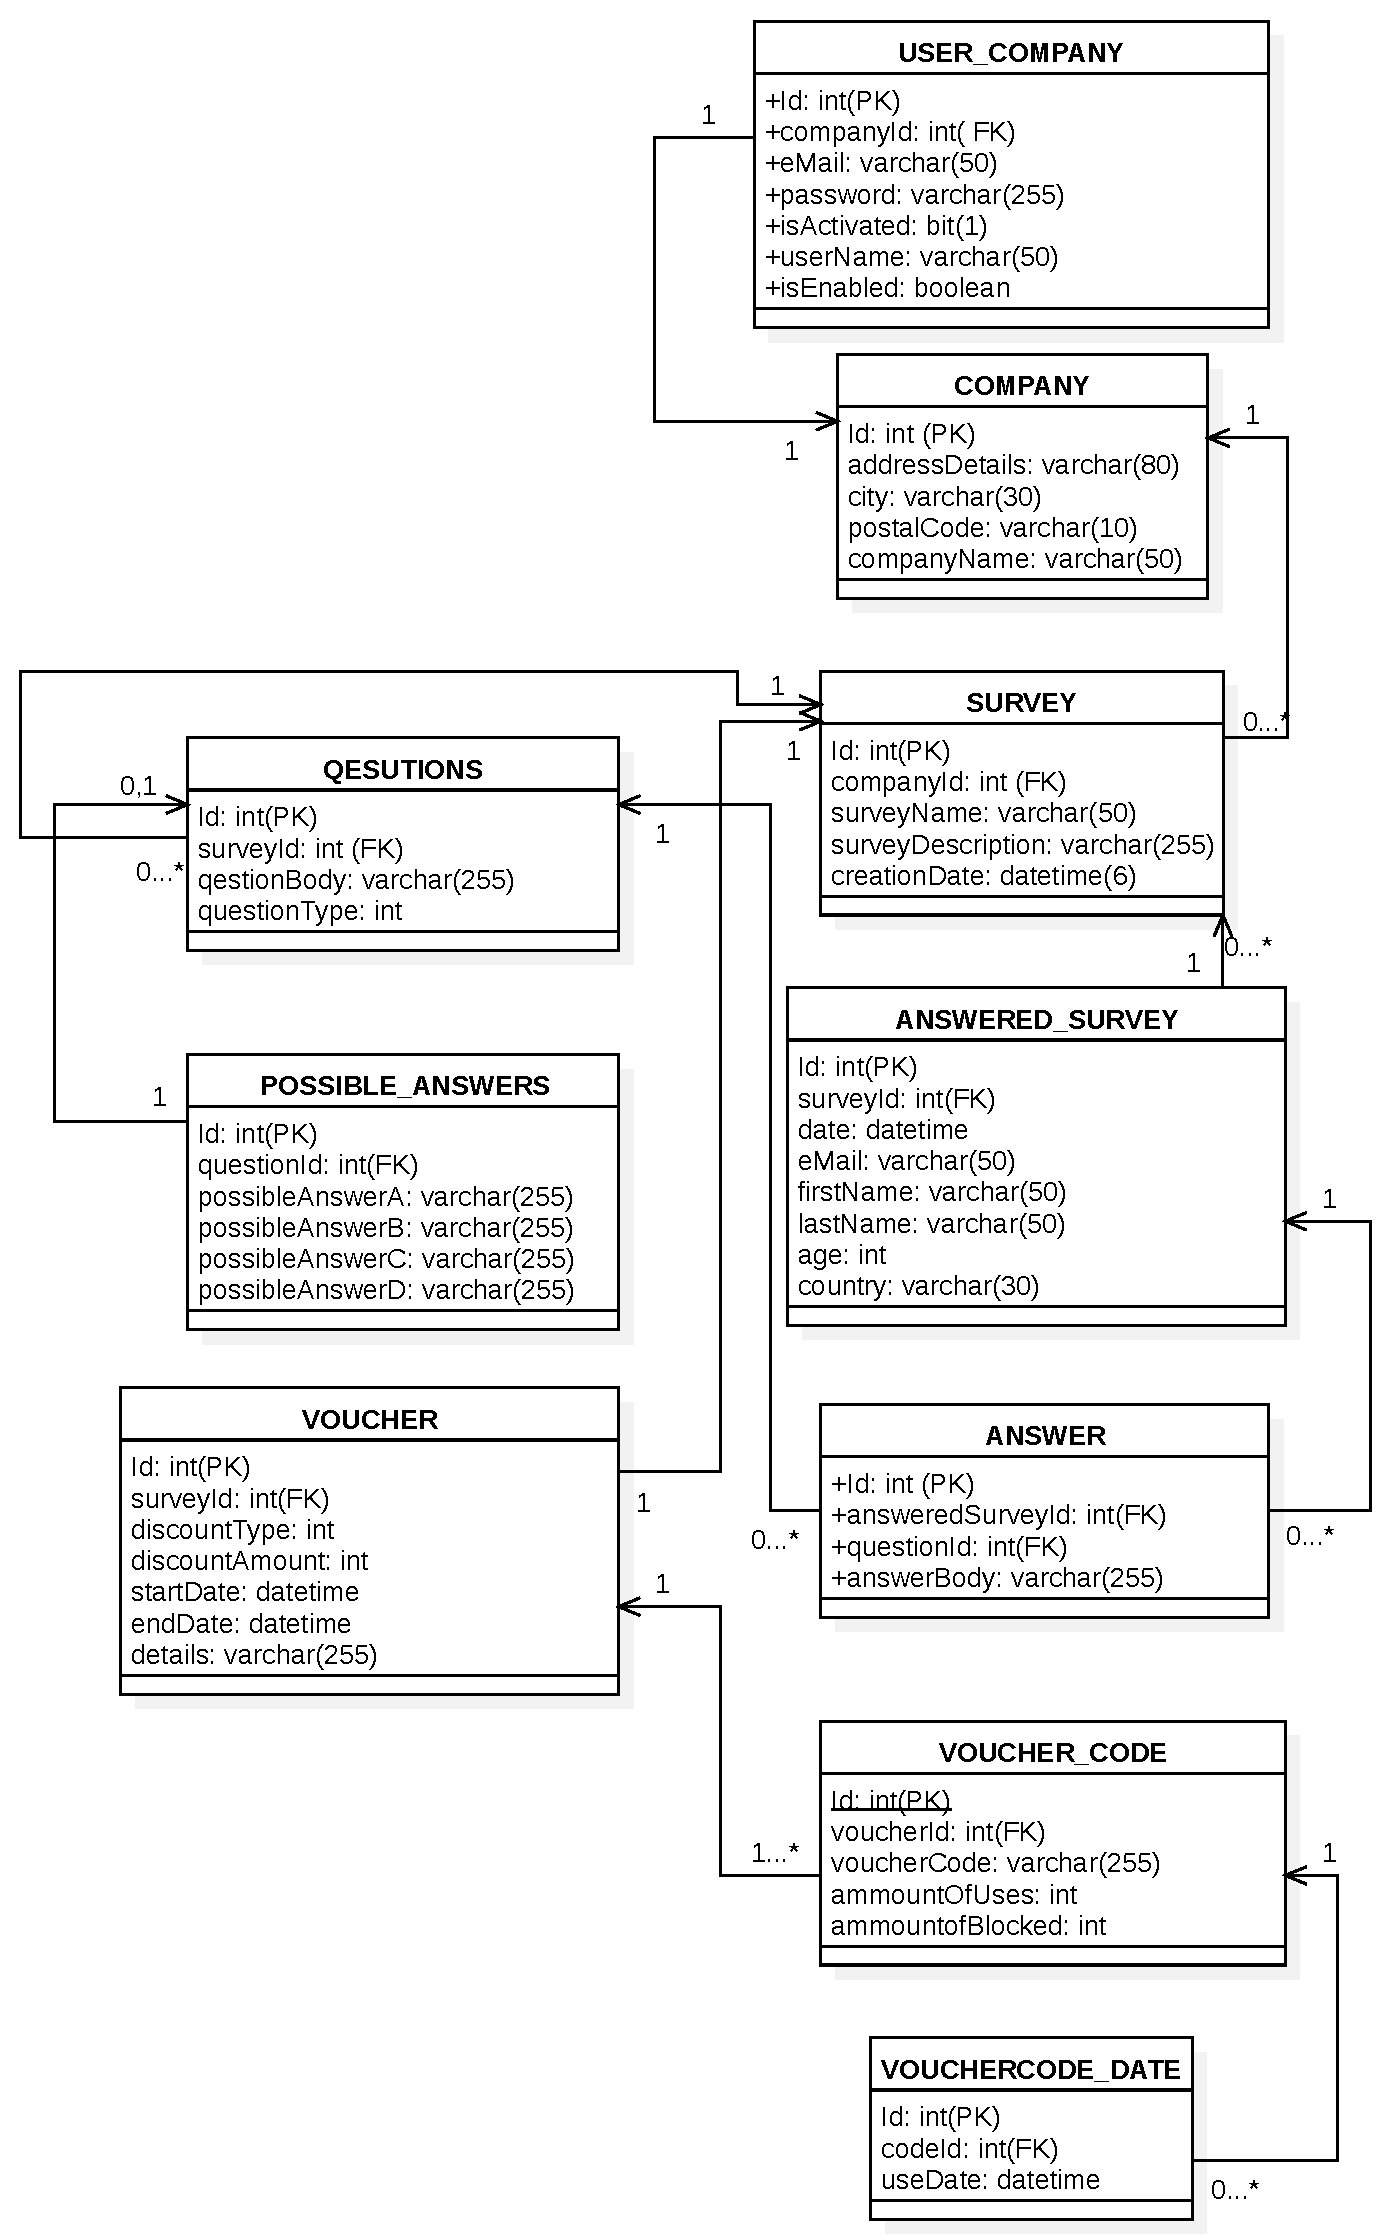
\includegraphics[scale=0.55]{db_diagram.pdf}
  \caption{Diagram klas przedstawiający baze danych systemu}
\end{figure}
W celu odpowiedniego zrozumienia struktury naszej aplikacji koniecznie jest zaznajomienie się kilkoma kluczowymi założeniami naszego systemu, którego miały bezpośredni wpływ na sposób w jaki zaprojektowaliśmy baze danych. Najważniejszym założeniem było przypisanie tylko i wyłącznie jednego typu kupony do jednej ankiety. Żadna ankieta może oferować tylko wyłacznie jeden typ kupony jako nagrodę za wypełnienie ankiety. Każdy voucher (który reprezentuje typ nagrody) może już miec przypisany więcej niż jeden kupon, każdy z nich może byc wielokrotnego użytku ( wtedy należy zaznaczyć jak wiele osób z niego może skorzystać) lub też jednorazowego użytku.

\paragraph{}
Równie ważnym założeniem było stworzenie tablicy \textbf{VoucherCode\_Date}, który odpowiada za ``blokowanie'' kupony na czas wypełnienia ankiet.
\subsection{Opis protokołów}
Ruch po naszej aplikacji ma miejsce przy użyciu protokołu \textbf{TLS}. Co ważne dostęp do każdej podusługi lub też podstrony naszego systemu wymaga połączenia zabezpieczonego, a użytkwonik chcący korzystać z naszej aplikacji przy użyciu protokołu \textbf{HTML} jest automatycznie przekierowywany na odpowiednią strone, która wykorzystuje już \textbf{TLS}. Podobno sytuacja ma miejsce z aplikacją mobilną, której połączenie z serwerem ma miejscu przy użyciu \textbf{TLS}.

\paragraph{}
Część aplikacji webowej dbająca o uwierzytelnianie	oraz autoryzacje (ang. authentication and authorization) przychodzących połączeń są filtry, które możemy uznać za protokół. Są one częścią \textbf{Servlet'ów}, która ma za zadanie jak sama nazwa wskazuje filtrować przychodzące zapytania, jak również w zależności od samego zapytania w odpowiedni sposób reagować. Informacje zawarte w zapytaniach oraz odpowiedziach serwera, które zostają dynamicznie przechowycone przez filtry są wykorzystywane między innymi do tego aby zidentyfikować autora zapytania (autoryzacja) i jeżeli będzie taka konieczność nadać mu odpowiednie uprawnienia (uwierzytelnienie). Jednym z zaimplementowanych przez nas zabezpieczeniem jest autoryzacja na poziomie metod serwisowych, jak również nadawanie ról użytkownikom w zależności od typu uprawnienień, które posiadają. Każdej osboie korzystającej z naszej aplikacji zostaje nadany unikatowy indetyfikator sesji, którym zostaje powiązany on i uprawnienia, które posiada. Właśnie te informacje wykorzystuje \textbf{The Security Filter Chain}, który jest częścią jednego z używanych przez nas narzędzi. Kiedy użytkownik legitymuje się swoim identyfikatorem sesji \textbf{The Security Filter Chain} (od tego momentu nazywany filtrem w celu zwiększenia czytelności tekstu) sprwadza w bazie danych czy istnieje już powiązane z tym identyfikatorem połączenie, w przypadku gdy zostanie to potwierdzone filter sprawdza jakie uprawnienia posiada to połączenie, skutkuje to powiązaniem uwierzytelnieniu zapytania przychodzącego do serwera, co następnie umożliwia wykorzystanie autoryzacji na poziomie metod, która sprawdza czy nasze uprawnienia są wystarczające.

\paragraph{}
Każdy użytkownik aplikacji webowej posiada odgórnie pewne uprawnienia, a w przypadku zalogowania się następuje dodatkowe uwierzytelnienie, gdzie jego identyfikator sesji wiązany z kontem do którego jest aktualnie zalogowany. To właśnie dzięki temu filter bezpieczeństwa potrafi jednoznacznie potwierdzić czy przychodzące zapytanie legitymujące się jedynie identyfikatorem sesji ma wystarczające uprawnienia do danej podusługi.

\paragraph{}
Ze względu na taki a nie inny sposób uwierzytelniania oraz autoryzacji konieczne również było użycie dodatkowego zabezpieczenia w postaci losowych tokenów chroniących przed atakami \textbf{CSRF} (ang. Cross-site request forgery), które w trakcie generowania zostają powiązane z identyfikatorem sesji, na którego życzenie zostały wygenerowane. Każdy użytkownik naszego serwisu podczas zapytań typu \textbf{POST} (sytuacja taka ma najczęściej miejsce podczas zatwierdzaniu różnego typu danych do serwera) musi ``wylegitymować się'' wygenerowanym wcześniej dla niego \textbf{CSRF tokenem} jak również identyfikatorem sesji, dopiero wtedy filter bezpieczeństwa zatwierdza takie zapytanie i przekazuje je do warstwy kontrolerów.

\paragraph{}
Częścią naszego systemu jest serwis mailowy, przez który jesteśmy w stanie komunikować się z klientami. Korzysta on z protkołu \textbf{STMP}.

\subsection{Możliwości rozwoju systemu}
\paragraph{Wdrożenie systemu}
Po zbudowaniu aplikacji i dodaniu artefaktu w \texttt{IDE} generujemy plik \texttt{JAR} lub \texttt{WAR}, który można wdrożyć w chmurze, np. \textit{Amazon Web Services}, które po skonfigurowaniu \texttt{Load Balancera} pozwoli na korzystanie z wersji \textit{live} aplikacji webowej.

Aby wdrożyć aplikację mobilną należy utworzyć konto deweloperskie w serwisie \textit{Google Play}, a następnie wygenerować klucze dla aplikacji mobilnej, powiązać je z aplikacją mobilną i przesłać pliki aplikacji do serwisu \textit{Google'a}.

\paragraph{}
System gwarantuje całkowite pokrycie wszystkich założeń funkcjonalnych i niefunkcjonalnych. Możliwe jest jednak rozwój systemu o kolejne funkcjonalności. Bezpośrednimi funkcjonalnościami, które w łatwy sposób mogą zostać zbudowane na bazie istiejących rozwiązań są między innymi powiązanie kodów promocyjnych kuponu z kodami QR. Aby wprowadzić taką funkcjonalność będzie należało dodać kolejne pole w klasie odpowiadającej w modelu za kupon, które będzie przechowywać kod QR. Kod ten może być w łatwy sposób zwracany do użytkownika i wyświetlany na ekranie wraz z pozostałymi szczegółami kuponu. Kolejną funkcjonalnością, o którą może zostać rozbudowany system jest wprowadzenie algorytmu decydującego o zdobywaniu kuponu. Kupony mogą być wydawane co piąte wypełnienie ankiety, z dowolnym prawdopodobieństwem lub w ogóle. System jest napisany w sposób, który umożliwia modyfikacje serwisu bez konieczności przeprojektowania pozostałej logiki. System charakteryzuje się wysoką spójnością i niskim sprzężęniem.

\chapter{Dokumentacja kodu}

\section{Użyte technologie}
Całość systemu została zaimplementowana w jęzku obiektowym \textbf{Java 8} przy użyciu narzędzi dostępnych w \textbf{Java EE} (ang. enterprise edition). Do automatyzacji budowania projektu w przypadku aplikajci webowej został wykorzystany \textbf{Maven}, natomiast jeśli chodzi o aplikacje webową był to \textbf{Gradle}. Framework w oparciu którego została napisana aplikacja mobilna jest \textbf{Retrofit}. Ułatwia on w znaczny sposób pracę z różnego typu HTML'owych API (ang. application programming interface), m.in REST API. Narzędzie w znaczny sposób ułatwiło nam mapowanie obiket na JSON'a oraz JSON'a na obiekty, jak również samo wysyłanie zapytań oraz odbieranie i interpretacja odpowiedzi serwera, pamietając o konieczności legitymacji się identyfikatorem sesji.

\paragraph{}
Jeśli chodzi o część systemu odpowiedzialną za aplikacje webową technologiami, które zostały wykorzystane są narzędzia z rodziny \textbf{Spring}. Program został zaprojektowany zgodnie z zasadami \textbf{GRASP},a podczas implementacji z zachowaniem tych zasadł pomógł nam \textbf{Spring Core}, ułatwiał on wykorzystanie wzorca \textbf{DI} (ang. Dependency Injection), co skutkowało zachowaniem niskiego sprzężenia oraz wyskokiej spójności klas. Znaczna większość obiektów, które były wstrzykiwane poprzez \textbf{DI} były przedstawicielami wzorca projektowego \textbf{Singleton}, co skutowało zmniejszeniem zapotrzebania na zasoby komputera naszego serwera. Singletonami są wszystkie klasy serwisowe, kontrolery oraz klasy konfiguracyjne. Poza klasami konfiguracyjnymi wszystkie klasy wstrzykiwane przy użyciu \textbf{Spring Core} były implementacjami interfesjów, co pozwoliło \textbf{Springowi} w bardzo lekki i łatwy sposób przy użyciu refleksji budowanie \textbf{Proxy} tych obiektów w trakcie uruchomienia aplikacji i załadowania kontekstu,a nie jak miałoby by to miejsce w przypadki gdyby obiekty wstrzykiwane rozszerzały klase (lub też nie rozserzały żadnej kalsy abstrakcyjnej) modyfikując kod bitowy, który został wcześniej skompilowany. W różnych częsiach projektu mieliśmy doczynienia z programowaniem aspektowym, które również było możliwe, dzięki \textbf{Spring Core} oraz wcześniej stworzonym \textbf{Proxy} do wstrzykiwanych klas. Framework, z którym najwięcej pracowaliśmy to \textbf{Spring MVC}. Jest to narzędzie, które umożliwia z jasny sposób budować aplikacje webowe w opraciu o wzorzec projektowy \textbf{MVC}. Dzięki niemu w łatwy sposób mogliśmy zbudować most łączący widok z modelem, czyli kontrolery. \textbf{Spring MVC} rownież ułatwił nam walidacje dancyh otrzymanych przez użytkowników poprzez pare na adnotacjach dostępnych w pakietach \textbf{javax.validation.api}. Wraz z \textbf{Spring MVC} wykorzystywany był \textbf{Jackson}, czyli biblioteka odpowiedzialana za mapowanie instancje klas na obiekty JSON, oraz w drugą stronę.

\paragraph{}
W zabezpieczaniu naszego systemu pomogły nam rownież \textbf{Spring Security} oraz \textbf{Spring Session}. Drugie z nich dawało nam większą kontrole nad sesjami i jej atrybutami (tak jak \textbf{CSRF tokeny} oraz blokowane kupony, które rownież wiązane były z sesją) jak również umożliwiało nam to przechowywanie identyfiaktorów sesji w bazie danych. Jeśli chodzi o \textbf{Spring Security} miał on wpływ na implementacja autoryzacji oraz uwierzytelniania w naszym serwisie. To narzędzie sprawdzało podczas otrzymania zapytania przez serwer, czy dany użytkownik legitymujący się identyfikatorem sesji ma odpowiednie uprawnienia do przeglądania danej podstrony jak również wywoływania metod zarówna w kontrolerze oraz w klasach serwisowych. Umożliwił w łatwy sposób również implementacje różnego typu handler'ów dla przypadków, gdy użytkownikowi nie udało się prawdiłowo zalogować/wylogować lub gdy właśnie probował przejść do strony, do której nie ma dostępu. Narzędzie to również automatycznie hashuje hasła podane przez użytkowników (po wcześniejszym zadeklarowaniu wybranego przez nas algorytmu haszującego), co jest znaczące jeśli chodzi o przechowywanie wrażliwych dla użytkoników danych.

\paragraph{}
Kolejnym narzędziem jest \textbf{Thymeleaf}, który został wykorzystanu do front-end'owej częsci projektu, czyli silnik umożliwiający tworzenie szablonów HTML, który jest w łatwy sposób jest integrowany ze \textbf{Spring MVC}.  Dzięki możliwości korzystania m.in. z pętl, branch'ów oraz fragmentów kod HTML'owy stworzony przy użyciu Thymeleafa jest spójny oraz czytelny, gdyż miejscami przypomina kod jakiegoś standardowego języka programowania. Podczas prac nad modelem zostały wykorzystane również : \textbf{JavaScript},\textbf{jQuery},\textbf{CSS}.

\paragraph{}
Przydatnym narzędziem okazały się również \textbf{Spring WebFlow} oraz \textbf{Spring Mail}, które oferują wysokopoziomowe interfejsy dla wielostopniowych formularzy (ang. wizards) oraz wysyłce maili o zadanych wcześniej wyglądach (szablonach HTML). Pełna integracja z kodem Javowym w narzędziu odpowiedzialnym za formularze jest nie do opisania, ponieważ dzięki temu w formularzach jesteśmy wstanie zastosować branche, pracować na wprowadzonych przez użytkownika danych, jak również je przetwarzać na każdym etapie wykonywania formualrza.

\paragraph{}
Narzędziami przez nas użytymi były rownież frameworki ORM (ang. Object-Relational Mapping), a chodzi tu o \textbf{Hibernate}. Poprzez właśnie to narzędzie następowała komunikacja z naszą bazą danych \textbf{MySQL}, czyli wprowadzanie,edycja oraz usuwanie danych. \textbf{Hibernate} odpowiedzialny był za mapowanie krotek bazodanowych na instacje klas Modelu oraz instacji klas modelu na zapytania SQL'owe. Wykorzystany został rownież do wygenerowania gotowej bazy danych, na której później pracowaliśmy.

\paragraph{}
Używamy również frameworka \texttt{caffeine}, który służy do cachowania. W naszym systemie są cachowane statystyki, które są elementem najbardziej obciążającym system. Cache ulega dezaktualizacji po 20 minutach i musi zostać wtedy odświeżony. Dodanie do systemu ankiety o danym \textit{id} powoduje również dezaktualizację cachu. Nie jest więc wykonywany niepotrzebny narzut pracy serwera, związany z dostarczaniem funkcjonalności statystyk w serwerze.

\section{Rejestracja}
\paragraph{}
Do implementacji mechanizmu rejestracji zostało wykorzystane narzędzie o nazwie \textbf{Spring WebFlow}, które jest wykorzystywane do wielostopniowego formularza (ang. wizard). W pliku XML-owym możemy odwoływac się do metod serwisowych, implementować na podstawie tego branch'e oraz decydowac na jakim etapie formularza jaka grupa walidacji będzie walidowana.
\begin{center}
\begin{lstlisting}[caption={Listing kodu odpowiedzialnego za rejestrację.},captionpos=b]
<?xml version="1.0" encoding="UTF-8"?>
<flow xmlns="http://www.springframework.org/schema/webflow"
      xmlns:xsi="http://www.w3.org/2001/XMLSchema-instance"
      xsi:schemaLocation="http://www.springframework.org/schema/webflow http://www.springframework.org/schema/webflow/spring-webflow-2.4.xsd">

    <var name="company" class="pwr.groupproject.vouchers.bean.form.NewUserCompanyForm"/>

    <view-state id="step1" view="/signup/signup1.html" model="company"
                validation-hints="'validationGroup1'" >
        <transition on="nextStep" to="step2">
            <evaluate expression="userCompanyServiceImpl.validateUserCompany(company,messageContext)" />
        </transition>
        <transition on="cancel" to="cancel" validate="false" bind="false" />
    </view-state>

    <view-state id="step2" view="/signup/signup2.html" model="company"
                validation-hints="'validationGroup2'">
        <transition on="nextStep" to="success">
            <evaluate expression="userCompanyServiceImpl.addUser(company)" />
        </transition>
        <transition on="cancel" to="cancel" validate="false" />
        <transition on="previousStep" to="step1" validate="false" />
    </view-state>

    <end-state id="success" view="externalRedirect:/?acc=1" />
    <end-state id="cancel" view="externalRedirect:/" />
</flow>
\end{lstlisting}
\end{center}
Dla pierwszego etapu rejestracji do modelu (który jest ten sam dla całego trwania procesu) dodawany jest pusty formularz, czyli obiekt w którym będziemy przechowywać wszystkie dane wprowadzone przez użytkownika. Następnie po zatwierdzeniu pierwszego etapu przez użytkownika , sprwadzamy czy wprowadzone dane są zgodne z wymogami przedstawionymi przez serwer (np. czy podany przez użytkownika adres e-mail nie znajduje się już w naszej bazie danych) poprzez $<evaluate expression="userCompanyServiceImpl.validateUserCompany(company,messageContext)" />$,  w której wywołujemy klase serwisową naszego systemu. W przypadku, gdy dane nie spełnią wymogów wyświetlamy odpowiednie komunikaty błędów, w których jasno informujemy klienta co należy zrobić, aby owe wymogi spełnić. W przypadku gdy dane zostaną zatwierdzone przez serwer przechodzimy do drugiego etapu formularza  $<view-state id="step2" ... </view-state>$. Tam użytkownik uzupełnia formularz kolejną serią danych (np. hasłem oraz jego powtórzeniem) po zatwierdzeniu których serwer poraz kolejny waliduje dane wejściowe, tym razem już cały formularz. W przypadku przejścia wszystkich wymogów walidacji zostaje wykonana instrukcja $<transition on="nextStep" to="success">...</transition>$, co skutkuje wywołanem funkcji serwisowej $addUser(obj: Company)$. Po pomyślnym dodaniu użytkownika do bazy danych proces trafia do linijki $25$ w powyższym listingu i zostaje przekierowany na strone startową, na której dzięki parametrowi ``acc'' wyświetli się odpowiedni komunikat informujący o konieczności aktywacji konta przed zalogowaniem się.


\section{Resetowanie hasła dla konta}
\paragraph{}
\begin{center}
\begin{lstlisting}[caption={Listing kodu obsługującego odzyskiwanie hasła.},captionpos=b]
@RequestMapping(value = "forgot_password", method = RequestMethod.GET)
public String forgottenPassword(Model model) {
	model.addAttribute("form", new ForgotPasswordForm());
	return "auth/forgot_password.html";
}

@RequestMapping(value = "forgot_password", method = RequestMethod.POST)
public String forgottenPassword(@ModelAttribute(name = "form") @Validated ForgotPasswordForm forgotPasswordForm, BindingResult bindingResult) {
	if (bindingResult.hasErrors())
		return "auth/forgot_password.html";

	UserCompany userCompany = userCompanyService.getUserByUserName(forgotPasswordForm.getUserName());
	if (userCompany == null) {
		bindingResult.rejectValue("userName", "email.dont.exist", messageSource.getMessage("message.wrong.email", null, LocaleContextHolder.getLocale()));
		return "auth/forgot_password.html";
	} else if (!userCompany.isEnabled()) {
		bindingResult.rejectValue("userName", "account.not.activated", messageSource.getMessage("messages.account.not.activated", null, LocaleContextHolder.getLocale()));
		return "auth/forgot_password.html";
	} else {
		PasswordResetToken passwordResetToken = tokenService.generateNewPasswordResetToken(userCompany);
		mailService.sendPasswordResetEmail(passwordResetToken.getToken(), userCompany.getUsername());
	}

	return "redirect:/?acc=5";
}
\end{lstlisting}
\end{center}
Metoda oznaczona adnotacją $@RequestMapping(value = "/reset_password", method = RequestMethod.GET)$ przygotowywuje pusty formularz który ma zawierać jedynie adres e-mail konta dla którego użytkownik chce zresetować hasło. W przypadku, gdy użytkownik poda adres e-mail, który faktycznie znajduje się w naszej bazie danych zostaje generowany jednorazowy token (co zostało przedstawione w listingu poniżej), który zostaje wysłany w mail'u na wcześniej wskazany adres e-mail.

\begin{center}
\begin{lstlisting}[caption={Listing kodu generującego token do odzyskiwania hasła.},captionpos=b]
@Override
public PasswordResetToken generateNewPasswordResetToken(UserCompany userCompany) {
	tokenDao.deleteUsersResetTokens(userCompany.getUsername());
	PasswordResetToken passwordResetToken = new PasswordResetToken();
	passwordResetToken.setUserCompany(userCompany);
	passwordResetToken.setToken(RandomString.make(TOKEN_LENGTH));
	tokenDao.addPasswordResetToken(passwordResetToken);
	return passwordResetToken;
}

@Override
public PasswordResetToken validatePasswordResetToken(String passwordResetToken) throws WrongTokenException {
	try {
		return tokenDao.getPasswordResetTokenByToken(passwordResetToken);
	} catch (NoResultException ex) {
		throw new WrongTokenException();
	}
}
\end{lstlisting}
\end{center}
Tylko i wyłącznie jeden token odpowiadający za resetowanie hasła może być pisany do konta, tak więc przed dodaniem nowego ``PasswordResetToken'' ewentualny obiekt, który mógł istnieć wcześniej jest kasowany.

\begin{center}
\begin{lstlisting}[caption={Listing kodu resetującego hasło.},captionpos=b]
@RequestMapping(value = "/reset_password", method = RequestMethod.GET)
public String resetPassword(@RequestParam("t") String token, Model model) {
	try {
		tokenService.validatePasswordResetToken(token);
		ResetPasswordForm form = new ResetPasswordForm();
		form.setResetPasswordToken(token);
		model.addAttribute("resetPasswordForm", form);
		model.addAttribute("tokenStatus", TokenStatus.OK);
	} catch (WrongTokenException ex) {
		model.addAttribute("tokenStatus", TokenStatus.WRONG);
	}
	return "token/reset_password.html";
}

@RequestMapping(value = "/reset_password", method = RequestMethod.POST)
public String resetPassword(@ModelAttribute @Validated ResetPasswordForm resetPasswordForm, BindingResult bindingResult, Model model) {
	if (bindingResult.hasErrors()) {
		try {
			tokenService.validatePasswordResetToken(resetPasswordForm.getResetPasswordToken());
			model.addAttribute("tokenStatus", TokenStatus.OK);
		} catch (WrongTokenException ex) {
			model.addAttribute("tokenStatus", TokenStatus.WRONG);
		}
		return "token/reset_password.html";
	}
	userCompanyService.changePassword(resetPasswordForm);
	return "token/reset_password_success.html";
}
\end{lstlisting}
\end{center}
Użytkownik klikający w link w mailu wysłanym przez nasz system przekazujemy w postaci parametru zapytani $GET$ wcześniej wygenerowany token. Po wcześniejszej walidacji tokenu użytkwonik jest przeniesiony do strony zawierający formularz, w którym podaje dwa razy to samo nowe hasło, którym od momentu potwierdzenia formularza będzie się posługiwał.


\section{Tworzenie ankiety}
\paragraph{}
Proces tworzenia ankiety zaczyna się w momencie wysłania żądania \texttt{GET} przez zalogowaną firmę pod adres \texttt{/surveys/add}. Po stronie klienta jest wczytywany panel do tworzenia ankiety pozwalający na bieżącą edycję ankiety w trakcie jej tworzenia. Panel pozwala na dowolne zmiany nazwy, opisu ankiety oraz kolejności pytań. Jest możliwe również usuwanie poszczególnych pytań z ankiety. Możliwy jest również podgląd ankiety w czasie rzeczywistym. Do pól odpowiadających za nazwę oraz opis ankiety są podłączone słuchacze zdarzeń, które po zmianie wartości wspomnianych pól wywołują \textit{callback}, wprowadzający zmiany w podglądzie ankiety. Pytania w czasie tworzenia ankiety są przechowywane w tablicy obiektów w języku \texttt{Javascript}. Każde dodane pytanie ma podmienianą treść przy użyciu wyrażenia regularnego, dzięki czemu od strony front-endu pytania zabezpieczane są przed próbą wstrzyknięcia złośliwego skryptu. Dla znaków \texttt{"}, \texttt{'}, \texttt{/}, \texttt{<} oraz \texttt{>} są stosowane sekwencje ucieczkowe.

\paragraph{}
Po nacisnięciu przycisku \texttt{Dodaj ankietę}, do serwera wysyłane jest żądanie \texttt{POST} zawierające w ciele \texttt{JSON}, który jest automatycznie mapowany na obiekt z języka \texttt{Java}, dzięki zastosowaniu parsera \texttt{Jackson}. Obiekt klasy \texttt{SurveyDto} jest walidowany pod kątem zawartości niedozwolonych znaków oraz braku pól pustych. Jeżeli walidacja się powiedzie, do klienta jest zwracana odpowiedź ze statusem \texttt{HttpServlet\linebreak Response.SC\_CREATED} i po stronie klienta następuje przekierowanie do panelu zarządzania ankietami. W przypadku, gdy walidacja się nie powiedzie, do klienta zwracana jest odpowiedź ze statusem \texttt{HttpServlet\linebreak Response.SC\_NOT\_ACCEPTABLE} i następuje powiadomienie o niepowodzeniu dodania ankiety.

\paragraph{}
Po udanej walidacji obiektu klasy \texttt{SurveyDto} wywoływana jest metoda \texttt{addSurvey} z serwisu \texttt{Company\-Survey\-Service}, która dodaje utworzoną ankietę do bazy danych. Przed dodaniem ankiety do bazy danych, na podstawie obiektu \texttt{SurveyDto} jest tworzony obiekt klasy \texttt{Survey}, który jest integralną częścią modelu aplikacji. Dzięki zastosowaniu obiektów klasy \texttt{SurveyDto} do komunikacji z klientem, możliwe jest oszczędność na przesyle danych, gdyż do komunikacji nie są wykorzystywane niepotrzebne z punktu widzenia klienta dane, używane jednakże w bazie. Szybsza komunikacja została uzyskana kosztem narzutu pracy serwera, którą trzeba przeznaczyć na mapowanie obiektu klasy \texttt{SurveyDto} na obiekt klasy \texttt{Survey}.

\paragraph{}
Zmapowany obiekt klasy \texttt{Survey} jest w kolejnym kroku zapisywany w bazie danych, przy użyciu frameworka \texttt{Hibernate}. Framework ten pozwala na relacyjno-obiektowe mapowanie, dzięki czemu zobowiązanie do zapisania obiektu do bazy danych może być przesunięte na ten framework. Więcej o działaniu frameworka w projekcie można przeczytać w rodziale trzecim.

\begin{figure}[h]
\centering
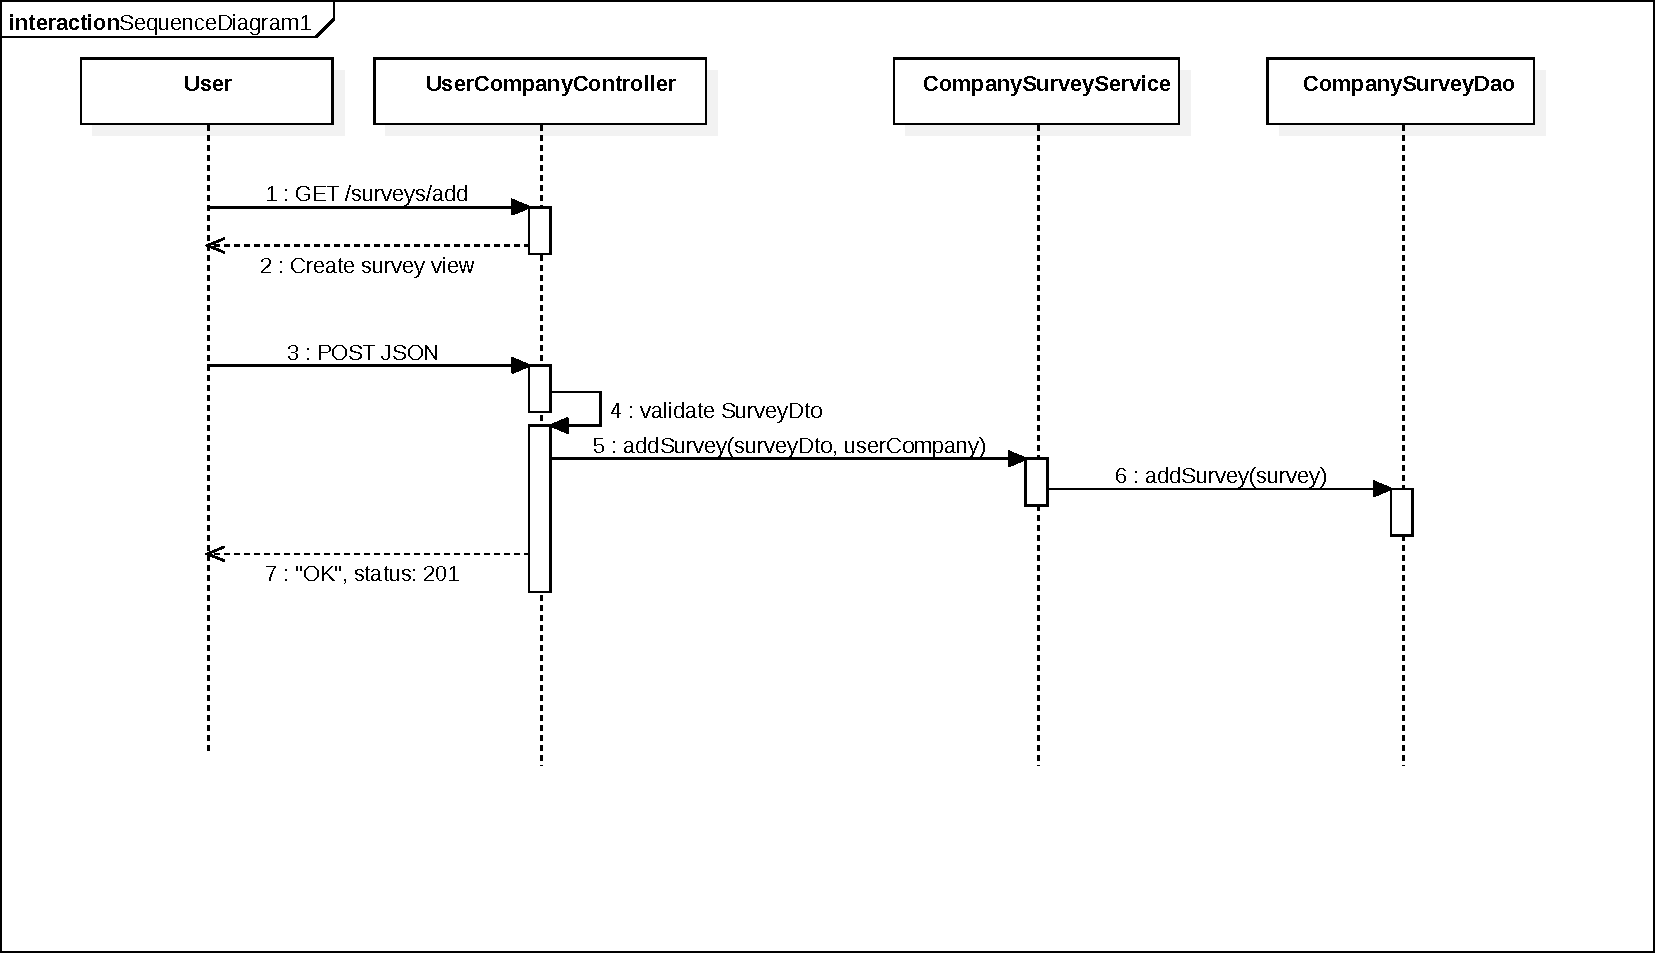
\includegraphics[width=15cm,height=20cm,keepaspectratio]{createSurveyPdf}
\caption{Diagram sekwencji dla poprawnego dodania nowej ankiety.}
\end{figure}

\paragraph{}
Na powyższym diagramie widoczne są połączenia między komponentami systemu dla dodawania nowej ankiety. Klasa \texttt{UserCompanyController} służy do komunikacji między użytkownikiem a resztą systemu. Walidacja zaznaczona na diagramie jako odwołanie \texttt{UserCompanyController} jest w rzeczywistości oddelegowana do walidatora, który dzięki zastosowanym w kodzie adnotacjom zna reguły walidacji pól w klasach. Oddelegowanie walidacji do walidatora jest oznaczone przy życiu adnotacji \texttt{@Validated} w argumencie kontrolera, który jest wiązany z ciałem żądania HTTP.

\section{Dodawanie kuponu}
\paragraph{}
Proces dodawania kuponu zaczyna się w momencie wysłania żądania GET przez zalogowaną firmę pod adres \texttt{/surveys/{id}/addVoucher}, gdzie {id} jest id wcześniej utworzonej ankiety. Po stronie klienta jest wczytywany panel do dodawania kuponu do wybranej ankiety. Panel pozwala na ustawienie rodzaju zniżki, jej wartości, opisu kuponu, a także czasu ważności kuponu.

\paragraph{}
Przy dodawaniu nowego kuponu tworzymy dane przypisywane do danego żądania i umieszczamy je jako atrybuty w \texttt{Modelu}. Dane te po wysłaniu odpowiedzi lub kolejnego żądania są wiązane z odpowiednimi obiektami w \texttt{Javie}. Dzięki takiemu rozwiązaniu można łatwo kontrolować walidację formularzy i łatwo sczytywać z nich dane, które następnie są procesowane w systemie.

\begin{center}
\begin{lstlisting}[caption={Listing kodu wywoływanego przy otrzymaniu żądania GET dla dodawania kuponu.},captionpos=b]
@RequestMapping(value = "/surveys/{id}/addVoucher", method = RequestMethod.GET)
    public String voucher(@AuthenticationPrincipal UserCompany userCompany, @PathVariable("id") int surveyId, Model model) {
        if(!checkForSurveyExistence(surveyId,userCompany)){
            return "error.html";
        }
        model.addAttribute("surveyId", surveyId);
        model.addAttribute("discountType", DiscountType.values());
        model.addAttribute("voucherForm",new VoucherForm());

        return "my_account/vouchers/add_voucher";
    }
\end{lstlisting}
\end{center}

W linijce pierwszej został określony mapping żądania \texttt{GET}. W linijkach 6-8 dodawane są atrybuty do modelu, które następnie będą zapełniane danymi, które dostarczy klient. W linijce 10 jako odpowiedź na żądanie jest zwracany HTML z widokiem panelu dodawania kuponu.

\paragraph{}
Po naciśnięciu przycisku \texttt{Zatwierdź}, do serwera wysyłane jest żądanie POST z obiektem \texttt{VoucherForm}. Obiekt klasy \texttt{VoucherForm} jest walidowany pod kątem zawartości niedozwolonych znaków oraz braku pól pustych. Jeżeli walidacja się powiedzie, do klienta zwracane są odpowiedzi analogicznie jak w przypadku procesu tworzenia ankiety.

\paragraph{}
Po udanej walidacji obiektu klasy \texttt{VoucherForm} wywoływana jest metoda \texttt{addVouchersForm} z serwisu \texttt{CompanySurveyService}, która dodaje utworzony kupon do bazy danych, łącząc go z odpowiednią ankietą. Zmapowany obiekt klasy \texttt{Voucher} jest w kolejnym kroku zapisywany w bazie danych, przy użyciu frameworka Hibernate. Proces dodawania kuponu jest zatem analogiczny, jak proces dodawania nowej ankiety.



\section{Wypełnianie ankiety}
\paragraph{}
Proces wypełniania ankiety zaczyna się od kliknięcia przez użytkownika przycisku \texttt{Wypełnij ankietę} na pasku nawigacyjnym. Użytkownik wybiera interesującą go firmę, a następnie ankietę. Ankiety są przedstawione w sposób jasno informujący o nagrodzie obowiązującej w zamian za jej wypełnienie. Wybranie ankiety blokuje jeden z kodów promocyjnych dla danego kuponu i wiąże go z identyfikatorem sesji użytkownika. Blokada kuponu dla użytkownika trwa przez 20 minut, a po upłynięciu tego czasu sesja wygaśnie i ankieta będzie musiała być wypełniona kolejny raz. 

\clearpage
\begin{center}
\begin{lstlisting}[caption={Listing kodu zwalniającego kod kuponu po wygaśnięciu sesji},captionpos=b]
@Override
    public void doFilter(ServletRequest request, ServletResponse response, FilterChain chain) throws IOException, ServletException {
        HttpServletRequest httpServletRequest = (HttpServletRequest) request;
        HttpSession session = httpServletRequest.getSession(true);
        Integer vDateId = (Integer) session.getAttribute("vCode");
        if (vDateId != null) {
            try {
                VoucherCodeDate voucherCodeDate = companySurveyService.getVoucherCodeDateById(vDateId);
                LocalDateTime localDateTime = LocalDateTime.now().minusMinutes(20);
                if (Date.from(localDateTime.atZone(ZoneId.systemDefault()).toInstant()).compareTo(voucherCodeDate.getUseDate()) > 0) {
                    session.removeAttribute("vCode");
                    companySurveyService.deleteVoucherCodeDate(vDateId);
                }
            } catch (Exception e) {
                if(!(e instanceof NullPointerException))
                    e.printStackTrace();
                session.removeAttribute("vCode");
            }
        }
        chain.doFilter(request, response);
    }
\end{lstlisting}
\end{center}

Powyższy listing prezentuje metodę z klasy \texttt{VoucherCodeFilter}. Filtr ten dodany jest do łańcucha filtrów, który jest rekurencyjnie przechodzony za każdym razem, gdy do serwera trafia żądanie. Po przejściu przez filtry otrzymujemy zmodyfikowane żądanie, które następnie jest procesowane przez \texttt{dispatcherServlet}, ustalający co to za żądanie i do jakiego adresu się odnosi. Filtry i \texttt{dispatcherServlet} są częścią frameworka \texttt{Spring Boot}. Po trafieniu żądania do filtra \texttt{VoucherCodeFilter} następuje sprawdzenie, czy w atrybutach sesji powiązanej z danym żądaniem znajduje się zablokowany kod kuponu. Jeżeli z identyfikatorem sesji związany jest jakiś kupon to w linijkach 8-10 sprawdzane jest czy nie minął czas przeznaczony na wypełnienie ankiety. Jeżeli czas został przekroczony to w linijkach 11-12 usuwane jest powiązanie sesji z kodem kuponu i kod wraca do puli.

\paragraph{}
Za proces wypełnienia ankiety i dostarczenia użytkownikowi kuponu odpowiada \texttt{Spring WebFlow}. W rozdziale trzecim zostało opisane działanie tego komponentu frameworku \texttt{Spring}. Służy on do tworzenia wieloetapowych formularzy, tzw. \textit{wizardów}. Dzięki zastosowaniu etapowego podejścia nie jest możliwe odwołanie się do adresu, który przekazuje kupon użytkownikowi, bez wcześniejszego wypełnienia ankiety. \texttt{WebFlow} umożliwia również kontrolę odblokowywania kuponów w przypadku, gdy użytkownik zrezygnuje z wysyłania ankiety. Po kliknięciu przycisku \texttt{Anuluj} w ankiecie wysyłane jest żądanie do serwera, które usuwa powiązanie kuponu z identyfikatorem sesji użytkownika. Gdy użytkownik zamknie okno przeglądarki kupon zostanie zwolniony dopiero po wygaśnięciu sesji.

\paragraph{}
Po każdym kroku formularza wypełniania ankiety, dane są walidowane. Nie jest możliwe przejście do kolejnego kroku, bez pozytywnej walidacji danych z poprzedniego etapu formularza. Do walidacji wypełnionej ankiety używana jest metoda \texttt{validate\-Answered\-Survey\-Form} z serwisu \texttt{Company\-Survey\-Service}.

\paragraph{}
Drugim krokiem formularza wieloetapowego jest podanie przez użytkownika danych statystycznych, takich jak wiek oraz kraj pochodzenia. Dane te również są walidowane. W tym kroku możliwe jest również podanie adresu e-mail, na który zostanie przesłany kupon. Jest to jednak pole opcjonalne, gdyż jednym z założeń niefunkcjonalnych aplikacji było zapewnienie użytkownikom anonimowości. W przypadku podania przez użytkownika adresu e-mail, wywoływana jest metoda \texttt{sendVoucherCodeEmail} z serwisu \texttt{mailService}, która przesyła kod na podany adres e-mail.

\begin{center}
\begin{lstlisting}[caption={Listing kodu wysyłającego e-mail.},captionpos=b]
private boolean send(String destinationEmail, String subject, Context ctx, 
				String eMailTemplate) {
        MimeMessage eMailMessage = mailSender.createMimeMessage();
        MimeMessageHelper eMailMessageHelper;
        try {
            eMailMessageHelper = new MimeMessageHelper(eMailMessage, true);
            eMailMessageHelper.setTo(destinationEmail);
            eMailMessageHelper.setSubject(subject);

            final String htmlContent = this.htmlTemplateEngine.
            					process(eMailTemplate, ctx);
            eMailMessageHelper.setText(htmlContent, true);
            mailSender.send(eMailMessage);
            return true;
        } catch (MessagingException e) {
            e.printStackTrace();
            return false;
        }
    }
\end{lstlisting}
\end{center}


Do wysyłania wiadomości e-mail przez system służy klasa \texttt{JavaMailSender}, która do komunikacji wykorzystuje protokół SMTP. Wszystkie wiadomości tworzone przez system, nie tylko te zawierające w sobie kupony promocyjne, są budowane w standardzie MIME. Framework \texttt{Spring} pozwala na łatwe tworzenie szablonów wiadomości e-mail, które można dynamicznie zapełniać zawartością w trakcie działania systemu. W powyższym listingu została przedstawiona metoda odpowiadająca za wysyłanie wiadomości e-mail w serwisie \texttt{MailService}. Na początku tworzony jest obiekt wiadomości w standardzie MIME, który jest następnie wypełniany wartościami takimi, jak adresat i nadawca. Zawartość wiadomości jest generowany przy użyciu silnika do szablonów pochodzącego z frameworka \texttt{Spring}. Przekazując do silnika szablonów kontekst wiadomości, zawierający niezbędne wartości, wykorzystywane przy dynamicznym tworzeniu treści maila, można w łatwy sposób uzyskać kod HTML, który następnie zostanie przesłany jako wiadomość do nadawcy.

\paragraph{}
Bezpośrednio przed wysłaniem do użytkownika kuponu wiadomością e-mail, bądź przed przekierowaniem użytkownika na stronę z kodem promocyjnym, następuje dodanie ankiety do bazy danych i usunięcie powiązania kuponu z identyfikatorem sesji. Dodanie wypełnionej ankiety do bazy danych jest przeprowadzane analogicznie, jak dodawanie kuponu lub ankiety. Obiekt jest zapisywany w bazie danych przy użyciu frameworka \texttt{Hibernate}, który zapewnia mapowanie relacyjno-obiektowe. Za usunięcie powiązania kuponu z identyfikatorem sesji odpowiada metoda \texttt{confirmAnsweringSurvey} z serwisu \texttt{CompanySurveyService}.
\clearpage

\begin{center}
\begin{lstlisting}[caption={Listing kodu blokującego kod promocyjny.},captionpos=b]
	@CacheEvict(value = {"surveyStat","ansList"},key = "#surveyId")
    @Override
    public VoucherCodeDto confirmAnsweringSurvey(Integer surveyId, 
    	AnsweredSurveyForm answeredSurveyForm, RequestContext requestContext) {
        HttpSession httpSession = ((HttpServletRequest) requestContext.getExternalContext().getNativeRequest()).getSession(true);
        Integer vCodeId = (Integer) httpSession.getAttribute("vCode");
        httpSession.removeAttribute("vCode");
        VoucherCode voucherCode = deployVoucherCode(vCodeId);
        String email = answeredSurveyForm.getEmail();
        if(email != null && !email.equals("")) {
            mailService.sendVoucherCodeEmail(voucherCode, email);
        }
        return new VoucherCodeDto(voucherCode);
    }
\end{lstlisting}
\end{center}

Powyższy listing pokazuje działanie metody odpowiedzialnej za dostarczenie kuponu do użytkownika i zwolnienie jego powiązania z identyfikatorem sesji. W linijkach 5-8 usuwane jest powiązanie kodu kuponu z identyfikatorem sesji, natomiast w linijkach 9-12 jest wysyłana wiadomość e-mail, o ile użytkownik podał opcjonalny adres e-mail. Metoda zwraca \texttt{Data Transfer Object} \texttt{VoucherCodeDto}, który następnie jest wyświetlany użytkownikowi po przekierowaniu. Warto również zwrócić uwagę na dezaktualizację cache'a po dodaniu nowej ankiety. Cache jest używany w systemie do przechowywania statystyk. Więcej o cache'u oraz statstykach można przeczytać w podrozdziale 4.6.

\begin{figure}[h]
\centering
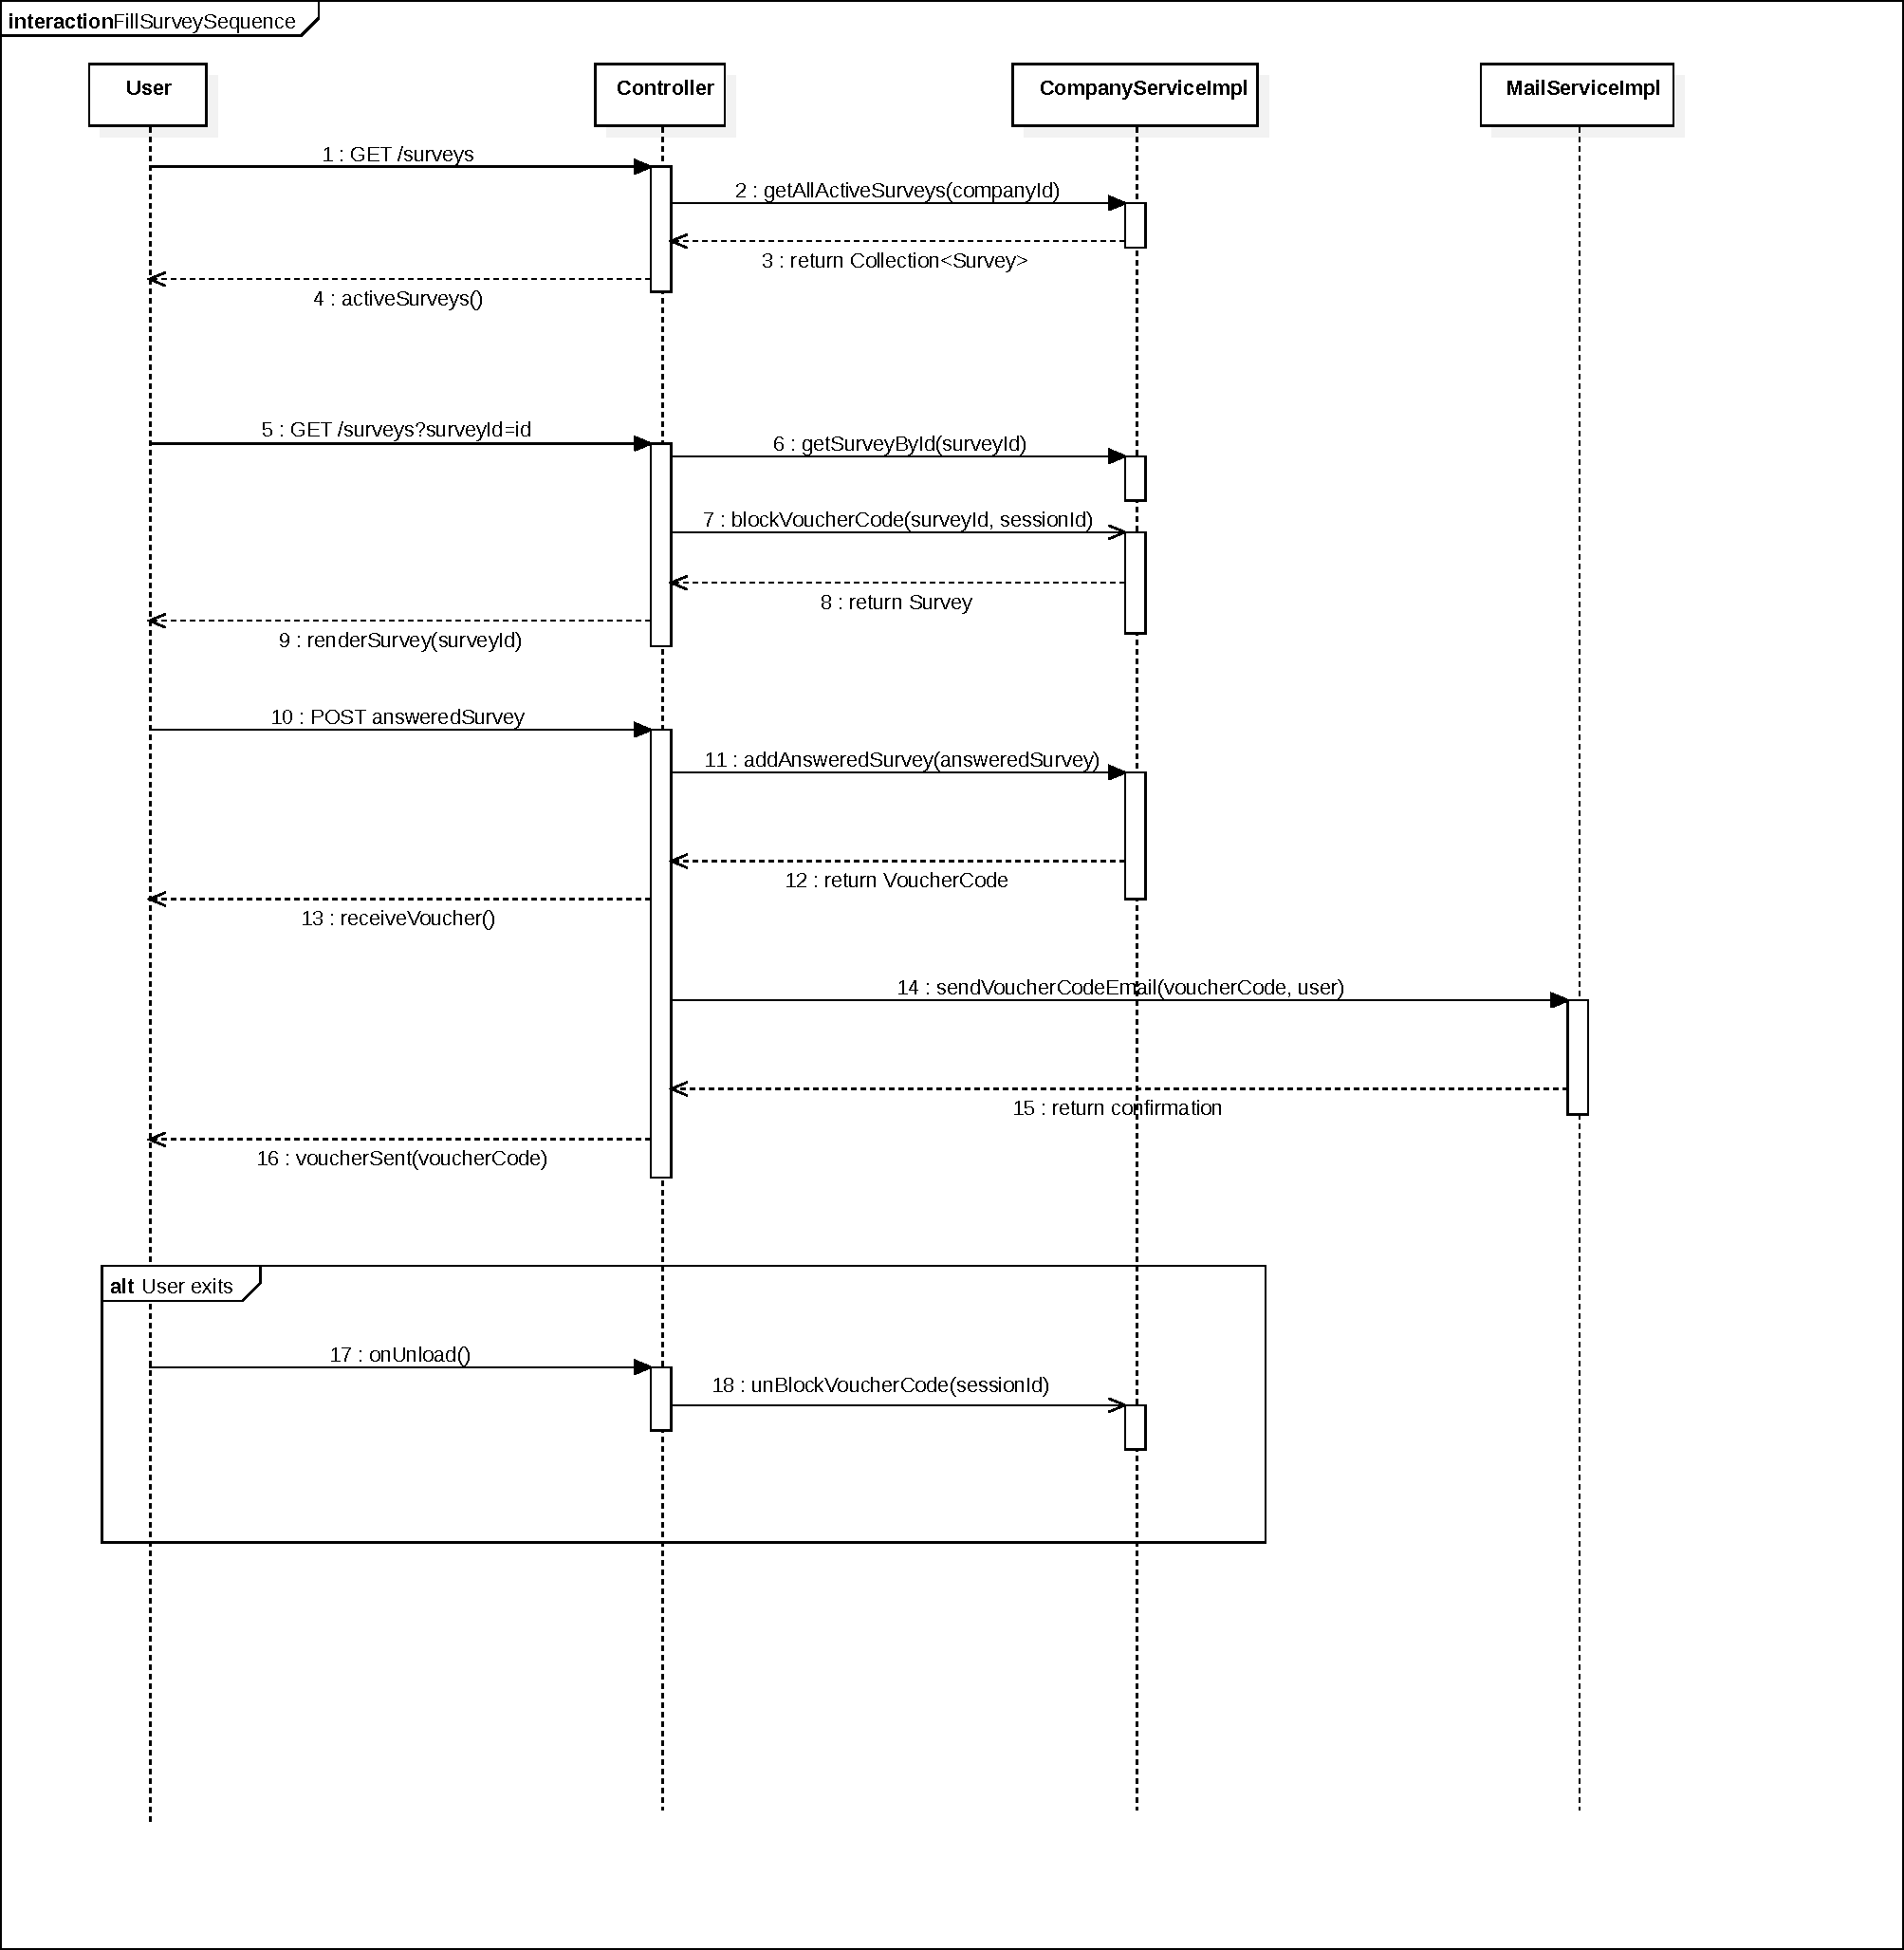
\includegraphics[width=10cm,height=10cm,keepaspectratio]{SequenceUMLFillSurvey}
\caption{Diagram sekwencji dla wypełniania ankiety.}
\end{figure}

Powyższy diagram sekwencji przedstawia proces wypełniania ankiety w aplikacji webowej. 

\section{Wypełnianie ankiety przez aplikację mobilną}
\paragraph{}
Aby móc wypełnić ankietę w aplikacji mobilnej, w tle wykonuje się wiele procesów zarówno aby dostarczyć odpowiednią ankietę do aplikacji mobilnej, jak i odpowiedzi udzielone przez użytkownika do serwera. Najpierw aplikacja mobilna, po wybraniu przez użytkownika firmy oraz ankiety, przesyła za pomocą frameworka retrofit2 metodą post informacje na temat interesującej użytkownika ankiety.
Serwer w momencie kiedy odbierze informacje, tworzy sesje dla naszej aplikacji, rezerwuje jeden kupon dla danego tokena sesji, oraz przesyła jako odpowiedź wyżej wymieniony token, wraz z pytaniami i typami pytań do konkretnie wybranej przez nas ankiety. Aplikacja mobilna odbierając plik JSON, zapisuje sobie plik cookie (który zapewnia nam utrzymanie sesji), oraz załącza pytania do listview w naszej nowo utworzonej aktywności. W trakcie dołączania pytań, aplikacja weryfikuje dla każdego z pytań jakiego jest ono rodzaju, i na tej podstawie tworzy kolejne elementy listview aby wyglądem pasowały do typu pytania. Na samym dole jest tworzony przycisk, służący do zaakceptowania naszej ankiety. Aplikacja w momencie gdy ankieta jest gotowa do wypełniania, umożliwia wysłanie ankiety dopiero wtedy, gdy zweryfikuje że odpowiedzi do ankiet są „niepuste”. 
Gdy użytkownik naciśnie przycisk akceptujący ankietę, i aplikacja dokona poprawnej walidacji ankiety następuje pobranie odpowiedzi z poszczególnych pól ankiety, umieszczenie ich w pliku JSON, oraz przesłanie ich metodą POST do serwera. Do naszej metody załączany jest plik cookies w którym przechowywany jest token sesji. W następnym kroku serwer przetwarza informacje przekazane przez aplikacje, zaś aplikacja czeka na odpowiedź z serwera. Jeżeli serwer nie był w stanie przetworzyć danych, (albo akurat w momencie gdy wysyłaliśmy nasza ankietę nie było zasięgu) nasza aplikacja mobilna informuje użytkownika o wystąpieniu błędu i cofa nas do ankiety. W przeciwnym przypadku serwer powinien zwrócić do aplikacji mobilnej plik JSON wraz z kodem promocyjnym oraz pozostałymi informacjami odnośnie otrzymanego vouchera. Gdy aplikacja odbierze wyżej wymieniony kod promocyjny, z automatu przekieruje nas do zakładki z posiadanymi kuponami.
W aplikacji mobilnej w zależności od tego czy podamy adres e-mail, możemy otrzymać kupon dodatkowo na konto e-mail. Warto dodatkowo zwrócić uwagę na fakt, że aplikacja została zaopatrzona w obsługę rezygnacji z wypełniania ankiety. Oznacza to, że w momencie gdy będziemy chcieli w aplikacji wrócić do menu głównego, albo zakończymy działanie aplikacji, to nasz program za pomocą metody POST wyśle informacje do serwera wraz z tokenem sesji o odblokowaniu vouchera który był dla nas wcześniej zarezerwowany.

\section{Statystyki}
\paragraph{}
\begin{lstlisting}[caption={Listing kodu pobierającego statystyki dla danej ankiety.},captionpos=b] 
@Cacheable("surveyStat")
@Override
public SurveyStatisticsDto getSurveysStatistics(int surveyId) {
	Collection<AnsweredSurvey> answeredSurveys = getAllAnsweredSurveysWithDetails(surveyId);
	Survey survey = companySurveyService.getSurveyByIdWithQuestion(surveyId);
	SurveyStatisticsDto surveyStatisticsDto = new SurveyStatisticsDto();
	surveyStatisticsDto.setAmmount(answeredSurveys.size());
	surveyStatisticsDto.setSurveyName(survey.getSurveyName());

	//average age
	double averageAge = answeredSurveys.stream().mapToInt(a -> a.getUser().getAge()).average().orElse(0.0);
	surveyStatisticsDto.setAge(averageAge);

	//average country
	List<String> countries = answeredSurveys.stream().map(a -> a.getUser().getCountry()).collect(Collectors.groupingBy(Function.identity(), Collectors.counting())).entrySet().stream().sorted(Comparator.comparingLong(Map.Entry::getValue)).limit(3).map(Map.Entry::getKey).collect(Collectors.toList());
	while (countries.size() != 3)
		countries.add("N/A");
	surveyStatisticsDto.setCountry(countries.toArray(new String[3]));
	
	if (answeredSurveys.size() == 0)
		return surveyStatisticsDto;

	//initialaizing iterators
	Iterator<AnsweredSurvey> answeredSurveyIterator = answeredSurveys.iterator();
	Iterator<Question> qIterator = survey.getQuestions().iterator();
	Iterator<Answer>[] aIteratorArray = new Iterator[answeredSurveys.size()];
	IntStream.range(0, aIteratorArray.length).forEach(i -> aIteratorArray[i] = answeredSurveyIterator.next().getAnswersList().iterator());

	int answersSize = answeredSurveys.size();
	List<QuestionStatisticsDto> questionStatisticsDtoList = surveyStatisticsDto.getQuestionWithAnswersList();
	while (qIterator.hasNext()) {
		Question q = qIterator.next();
		QuestionType qType = q.getQuestionType();
		QuestionStatisticsDto questionStatisticsDto = new QuestionStatisticsDto();
		questionStatisticsDto.setQuestionBody(q.getQuestionBody());
		questionStatisticsDto.setQuestionType(qType);

		switch (qType) {
			case OPEN:
				Arrays.stream(aIteratorArray).forEach(Iterator::next);
				questionStatisticsDto.setAnswers(null);
				break;
			case RANGED:
				double average = 0;
				for (Iterator<Answer> anAIteratorArray : aIteratorArray) {
					String temp = anAIteratorArray.next().getAnswer();
					average += Double.parseDouble(temp);
				}
				questionStatisticsDto.getAnswers()[0].setAnswersStat(Double.toString(average / answersSize));
				break;
			default:
				double[] apperances = new double[4];
				for (Iterator<Answer> anAIteratorArray : aIteratorArray) {
					Answer a = anAIteratorArray.next();
					String[] splited = a.getAnswer().split(",");
					for (String s : splited) {
						switch (s) {
							case "A":
								apperances[0]++;
								break;
							case "B":
								apperances[1]++;
								break;
							case "C":
								apperances[2]++;
								break;
							case "D":
								apperances[3]++;
		           		}
					}
				}
				IntStream.range(0, apperances.length).forEach(a -> questionStatisticsDto.getAnswers()[a].setAnswersStat(Double.toString(100 * apperances[a] / answersSize)));
				questionStatisticsDto.setPossibleAnswers(q.getPossibleAnswers());
				break;
		}
            
		questionStatisticsDtoList.add(questionStatisticsDto);
	}
	return surveyStatisticsDto;
}
\end{lstlisting}
Na powyższym listingu warto zauwazyć, że metoda jest cache'owana tj. zapmietywane jest przez serwer wartość, która zostanie zwrócona dla danego argumentu. Przy dużej liczbie rozwiązanych ankiet obliczanie statystyk, może być stosunkow czasochłonne, a sam cache zapewnia nam, że nie statystyki dla tych samych danych nie będa liczone kilkukrotnie.
\paragraph{}
Pierwszym etapem jest pobranie z bazy danych listy wypełnionych ankiet, a następnie policzenie średniego wieku przy użyciu \textbf{Stream API}, \textbf{Lamba Expressions} oraz klasy generycznej \textbf{Optional<T>}. Przy użyiu tych samych ``narzędzi'' dostępnych w Javie zostaje obliczona posortowana lista krajów, względem częstości wypełniania danej ankiety w tym kraju. Lista ta jest ograniczona do $3$ najlepszych wyników, a w przypadku gdy zawiera ona mniej niż $3$ kraje zostaje wypełniona wyrażeniem ``N/A''. W przypadku gdy ankieta nie została rozwiązana zwracany jest pusty obiad, w innej sytuacji w pętli iterujemy po pytaniach w kolejnych odpowiedziach, tzn. na początku dla każdej odpowiedzi na pytanie numer $1$ liczymy statystyki, następnie robimy to dla każdej istniejącej odpowiedzi na pytanie numer $2$ itd. Jeżeli pytanie jest pytaniem typu ``ranged'' (tj. w skali od 0 do 10) liczona jest średnia arytmetyczna wyniku. Jeżeli jest to pytanie typu zamkniętego lub zamkniętego wieloktronego wyboru przy pomocy \textbf{Stream API}, \textbf{Lamba Expressions} oraz klasy generycznej \textbf{Optional<T>} liczona jest częstość występowania danej odpowiedzi (która należy do zbioru $\{A,B,C,D\}$). Następnie przy pomocy set'erów i get'erów klasy \textbf{SurveyStatisticsDto} obliczone wcześniej dane zostają ``wrzucone'' do obiektu wyjściowego, który jest ostatecznie zwracany przez metode.


\end{document}